%\documentclass{beamer}
%\usepackage{lmodern} 
%
%\newcommand{\bsigma}{\mbox{\boldmath$\sigma$}}
%\newcommand{\bD}{\mbox{\boldmath$D$}}
%\newcommand{\bC}{\mbox{\boldmath$C$}}
%\newcommand{\bK}{\mbox{\boldmath$K$}}
%\newcommand{\bP}{\mbox{\boldmath$P$}}
%\newcommand{\bzero}{\mbox{\boldmath$0$}}
%\newcommand{\bB}{\mbox{\boldmath$B$}}
%\newcommand{\bu}{\mbox{\boldmath$u$}}
%\newcommand{\bv}{\mbox{\boldmath$v$}}
%\newcommand{\bg}{\mbox{\boldmath$g$}}
%\newcommand{\ba}{\mbox{\boldmath$a$}}
%\newcommand{\bb}{\mbox{\boldmath$b$}}
%\newcommand{\bx}{\mbox{\boldmath$x$}}
%\newcommand{\bbf}{\mbox{\boldmath$f$}}
%\newcommand{\bd}{\mbox{\boldmath$d$}}
%\newcommand{\bn}{\mbox{\boldmath$n$}}
%\newcommand{\bw}{\mbox{\boldmath$w$}}
%\newcommand{\bt}{\mbox{\boldmath$t$}}
%\newcommand{\bepsilon}{\mbox{\boldmath$\epsilon$}}
%\newcommand{\btau}{\mbox{\boldmath$\tau$}}
%\newcommand{\bnabla}{\mbox{\boldmath$\nabla$}}
%
%
%\usepackage{amsmath}
%\usepackage{graphicx,epstopdf}
%\usepackage[numberedbib]{apacite}
%\usepackage{bm}
%\usepackage{breqn}
%\usepackage{mathrsfs} 
%\usepackage{expl3}
%
%\DeclareMathOperator{\trace}{tr}
%\DeclareMathOperator{\divergence}{div}
%\DeclareMathOperator{\dist}{dist}
%\DeclareMathOperator{\dev}{dev}
%
%\let\cite\shortcite
%
%%\usetheme{default}
%%\usetheme{AnnArbor}
%%\usetheme{Antibes}
%%\usetheme{Bergen}
%%\usetheme{Berkeley}
%%\usetheme{Berlin}
%%\usetheme{Boadilla}
%%\usetheme{CambridgeUS}
%%\usetheme{Copenhagen}
%%\usetheme{Darmstadt}
%%\usetheme{Dresden}
%%\usetheme{Frankfurt}
%%\usetheme{Goettingen}
%%\usetheme{Hannover}
%%\usetheme{Ilmenau}
%%\usetheme{JuanLesPins}
%%\usetheme{Luebeck}
%%\usetheme{Madrid}
%%\usetheme{Malmoe}
%%\usetheme{Marburg}
%%\usetheme{Montpellier}
%%\usetheme{PaloAlto}
%%\usetheme{Pittsburgh}
%%\usetheme{Rochester}
%%\usetheme{Singapore}
%%\usetheme{Szeged}
%%\usetheme{Warsaw}
%\usecolortheme{lily}
%\useoutertheme{infolines}
%
%\newcommand{\SectionOne}{Phase Field Formulation}
%
%%\title[GE-XFEM]
%%{Extended Finite Element Method with Global Enrichment}
%
%\title[Phase Field]{Phase field approach to fracture:\\ Towards variational integrator techniques}
%
%\author[Vahid~Z.Rad] 
%{Vahid Ziaei-Rad}
%\institute[] 
%{
%Facult\'{e} des Sciences, de la Technologie et de la Communication
%}

\documentclass{beamer}
\usepackage{lmodern} 

\newcommand{\bsigma}{\mbox{\boldmath$\sigma$}}
\newcommand{\bD}{\mbox{\boldmath$D$}}
\newcommand{\bC}{\mbox{\boldmath$C$}}
\newcommand{\bK}{\mbox{\boldmath$K$}}
\newcommand{\bP}{\mbox{\boldmath$P$}}
\newcommand{\bzero}{\mbox{\boldmath$0$}}
\newcommand{\bB}{\mbox{\boldmath$B$}}
\newcommand{\bu}{\mbox{\boldmath$u$}}
\newcommand{\bv}{\mbox{\boldmath$v$}}
\newcommand{\bg}{\mbox{\boldmath$g$}}
\newcommand{\ba}{\mbox{\boldmath$a$}}
\newcommand{\bb}{\mbox{\boldmath$b$}}
\newcommand{\bx}{\mbox{\boldmath$x$}}
\newcommand{\bbf}{\mbox{\boldmath$f$}}
\newcommand{\bd}{\mbox{\boldmath$d$}}
\newcommand{\bn}{\mbox{\boldmath$n$}}
\newcommand{\bw}{\mbox{\boldmath$w$}}
\newcommand{\bt}{\mbox{\boldmath$t$}}
\newcommand{\bepsilon}{\mbox{\boldmath$\epsilon$}}
\newcommand{\btau}{\mbox{\boldmath$\tau$}}
\newcommand{\bnabla}{\mbox{\boldmath$\nabla$}}

\newcommand{\SectionZero}{Phase Field Approaches to Fracture}
\newcommand{\SectionOne}{Phase Field Formulation in Dynamic Context}
\newcommand{\SectionTwo}{Phase Field Formulation in General Context}
\newcommand{\SectionThree}{Phase Field Formulation with Incompressibility}
\newcommand{\SectionFour}{Impelementation on FEniCs}
%\newcommand{\SectionFive}{To Calculate the Crack Opening}
%\newcommand{\SectionSix}{Conclusion and Future Work}

\usepackage{fancyvrb}
\usepackage{color}

\usepackage{media9}
\usetheme{Ilmenau}
\usecolortheme{seahorse}
\usepackage[numberedbib]{apacite}
\usepackage[english]{babel}
%\usepackage{cite}

\usepackage{hyperref}
\hypersetup{
	bookmarks=true,         % show bookmarks bar?
	unicode=false,          % non-Latin characters in Acrobat’s bookmarks
	pdftoolbar=true,        % show Acrobat’s toolbar?
	pdfmenubar=true,        % show Acrobat’s menu?
	pdffitwindow=false,     % window fit to page when opened
	pdfstartview={FitH},    % fits the width of the page to the window
	pdftitle={My title},    % title
	pdfauthor={Author},     % author
	pdfsubject={Subject},   % subject of the document
	pdfcreator={Creator},   % creator of the document
	pdfproducer={Producer}, % producer of the document
	pdfkeywords={keyword1, key2, key3}, % list of keywords
	pdfnewwindow=true,      % links in new PDF window
	colorlinks=false,       % false: boxed links; true: colored links
	linkcolor=red,          % color of internal links (change box color with linkbordercolor)
	citecolor=green,        % color of links to bibliography
	filecolor=blue,      % color of file links
	urlcolor=blue           % color of external links
}
%\usepackage{abntcite}

\DeclareMathOperator{\dev}{dev}

\usepackage{amsmath}
\usepackage{graphicx,epstopdf,subfigure}
\graphicspath{{../Figs/}, {../Figures/}, {../ThesisFigs/}, {../AllFigs/}}
\addmediapath{../GuangxiUPresentation/}
%\usepackage[numberedbib]{apacite}
\usepackage{bm}
\usepackage{breqn}
\usepackage{mathrsfs} 
\usepackage{expl3}
\usepackage{amsmath, mathrsfs, bm}%, refcheck}
\usepackage{multimedia}
\usepackage{tabularx}
\DeclareMathOperator{\trace}{tr}
\let\cite\shortcite
\usepackage[ruled, vlined]{algorithm2e}
\usepackage{enumerate}

%\usepackage{stackengine}

\usepackage{graphicx}
\usepackage{media9}

\DeclareMathOperator{\divergence}{div}
\DeclareMathOperator{\dist}{dist}
%\usetheme{default}
%\usetheme{AnnArbor}
%\usetheme{Antibes}
%\usetheme{Bergen}
%\usetheme{Berkeley}
%\usetheme{Berlin}
%\usetheme{Boadilla}
%\usetheme{CambridgeUS}
%\usetheme{Copenhagen}
%\usetheme{Darmstadt}
%\usetheme{Dresden}
%\usetheme{Frankfurt}
%\usetheme{Goettingen}
%\usetheme{Hannover}
%\usetheme{Ilmenau}
%\usetheme{JuanLesPins}
%\usetheme{Luebeck}
%\usetheme{Madrid}
%\usetheme{Malmoe}
%\usetheme{Marburg}
%\usetheme{Montpellier}
%\usetheme{PaloAlto}
%\usetheme{Pittsburgh}
%\usetheme{Rochester}
%\usetheme{Singapore}
%\usetheme{Szeged}
%\usetheme{Warsaw}
\usecolortheme{lily}
\useoutertheme{infolines}

\usepackage{tikz}
\usepackage{ocg-p}
\usepackage{blindtext}
%\usepackage{hyperref}
\usepackage{pgfplots, pgfplotstable}

%\title[GE-XFEM]
%{Extended Finite Element Method with Global Enrichment}

%\logo{\makebox[1\paperwidth]{
\includegraphics[width=1.0cm,keepaspectratio]{LOGO-ERC.pdf}}}
\usepackage{eso-pic}
\newcommand\AtPagemyUpperLeft[1]{\AtPageLowerLeft{%
		\put(\LenToUnit{0.9\paperwidth},\LenToUnit{0.85\paperheight}){#1}}}
\AddToShipoutPictureFG{
	\AtPagemyUpperLeft{{
\includegraphics[width=1.cm,keepaspectratio]{LOGO-ERC.pdf}}}
}%

\title[UM-SJTU JI]{Introduction to FEniCS}

\author[Vahid~Ziaei-Rad] 
{\textbf{Vahid~Ziaei-Rad}}
\institute[]
{
University of Michigan-Shanghai Jiao Tong University Joint Institute}
%\date{Nov. 21, 2019}

\begin{document}

\begin{frame}
\titlepage 
\end{frame}

\begin{frame}
	\frametitle{Prelude: Medical Simulations}
	\framesubtitle{\SectionZero}
	%	\vspace{\baselineskip}
	\begin{itemize}
		\setlength\itemsep{2em}
		\item The aim of ''RealTCut'' is to devise real-time numerical methods for the simulation of cutting. \cite{Courtecuisse2014394}
		\item These methods are aimed at surgical training, which has the potential to help surgeons improve their skills without endangering patients.
		\begin{figure}
			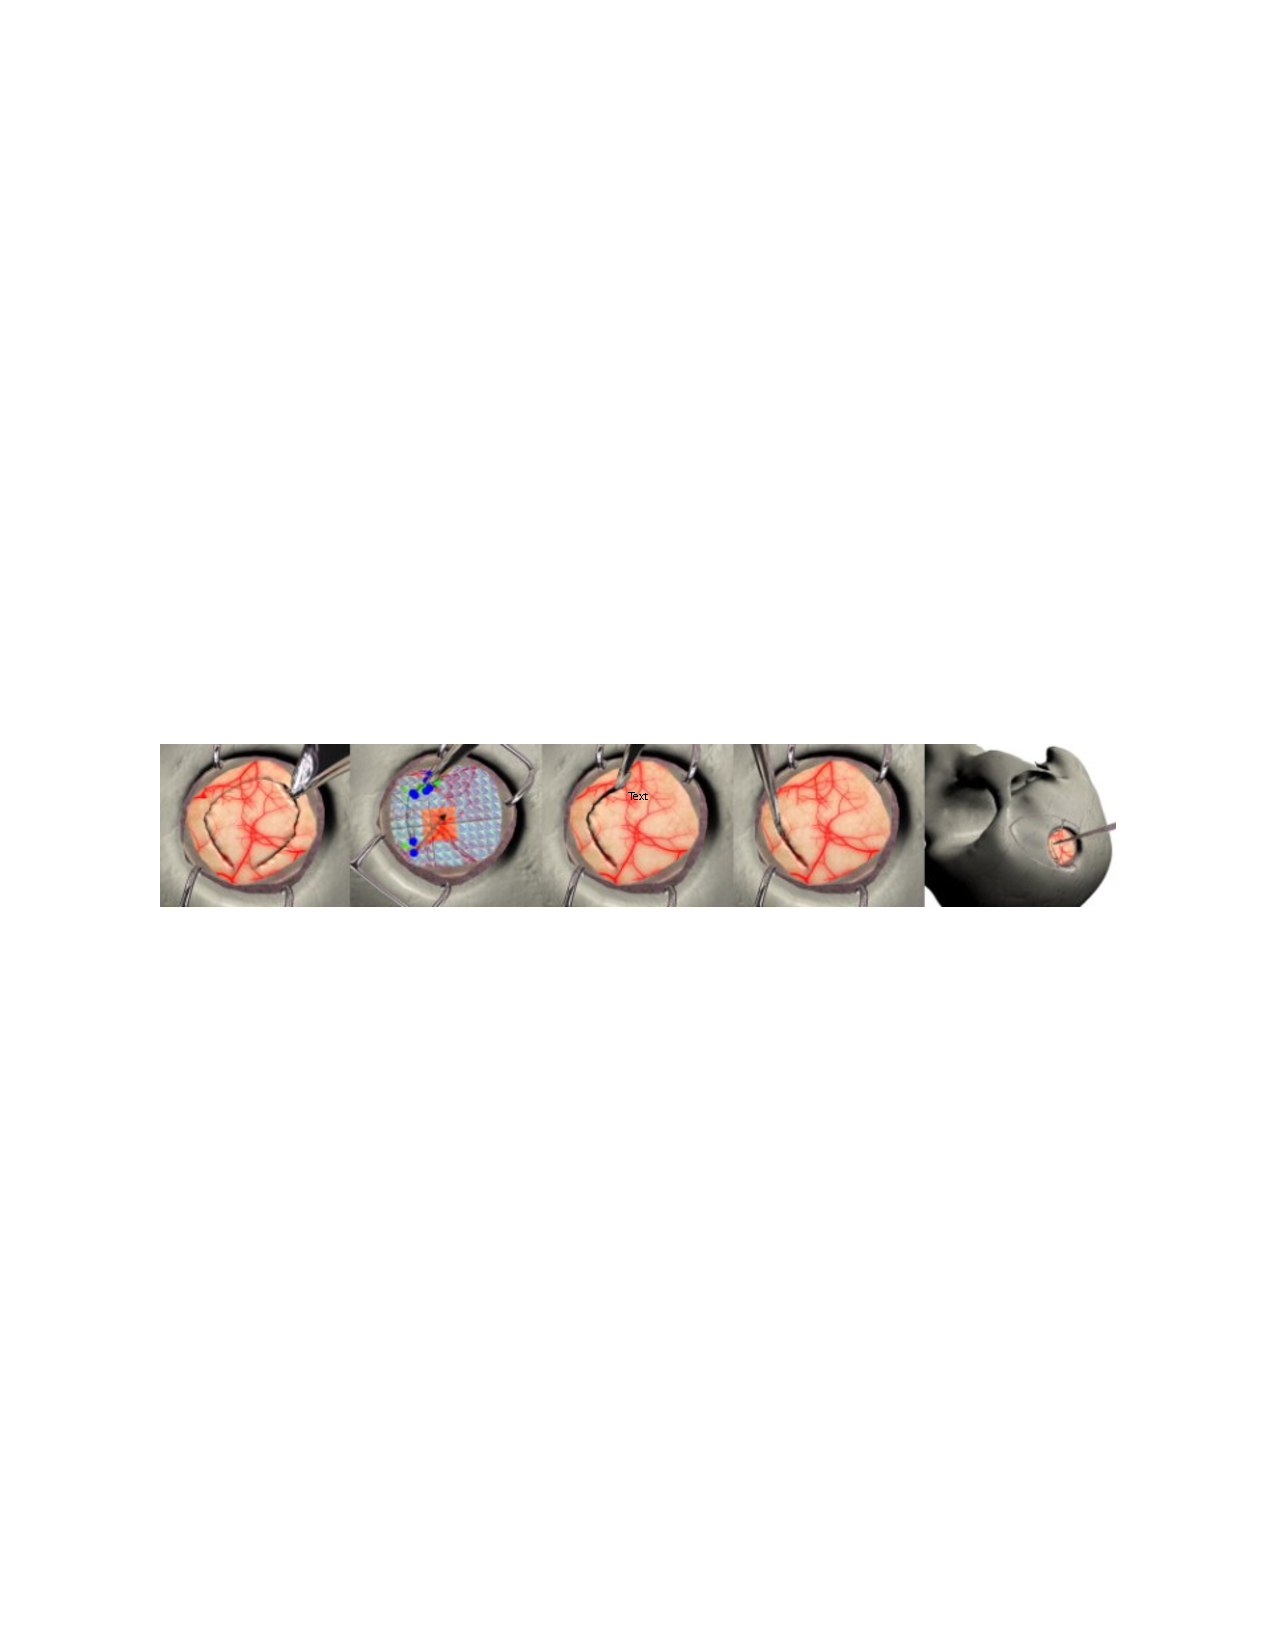
\includegraphics[width=.7\textwidth]{Medical.pdf}
		\end{figure}
		\item Here, we are more interested in predictive and accurate simulations\ldots
		\item We have some thoughts on phase field approaches to model fracture of ''incompressible'' soft tissues. \cite{Gultekin2016}
	\end{itemize}
\end{frame}

\begin{frame}
	\frametitle{Towards Real-Time Multi-Scale Simulation of Cutting}
	\framesubtitle{\SectionZero}
	\vspace{\baselineskip}		
		\begin{center}
			\includemedia[activate=onclick,
			width=0.4\textwidth
			]{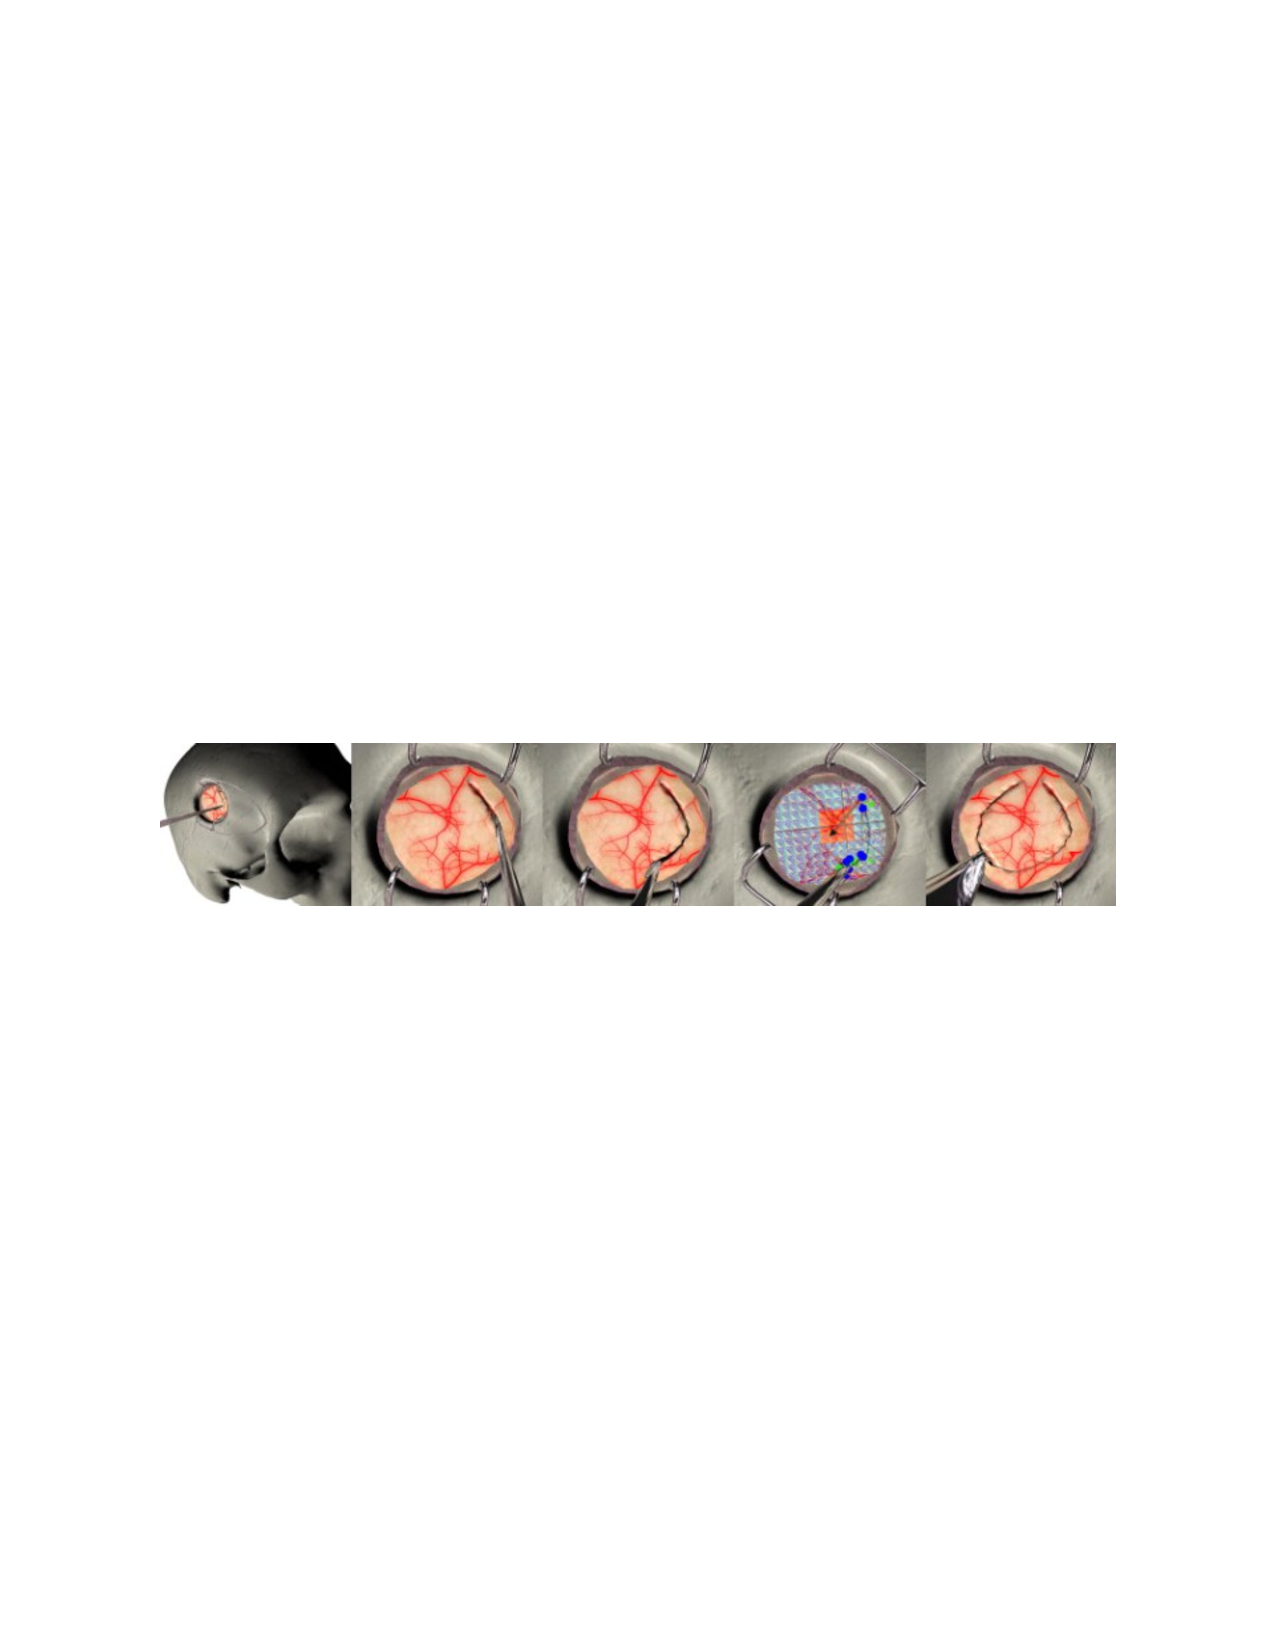
\includegraphics{Medicali.pdf}}{./Application.swf}
		\end{center}
\end{frame}

%\begin{frame}
%	\frametitle{Prelude: Explicit Crack Approaches}
%	\framesubtitle{\SectionZero}
%	%	\vspace{\baselineskip}
%	\begin{itemize}
%		\setlength\itemsep{2em}
%		\item The explicit crack approaches
%		\begin{itemize}
%			\item \textbf{Family 1:} To regenerate/adjust the mesh
%			\item \textbf{Family 2:} To introduce enrichment for the displacement discontinuity
%			\begin{figure}
%				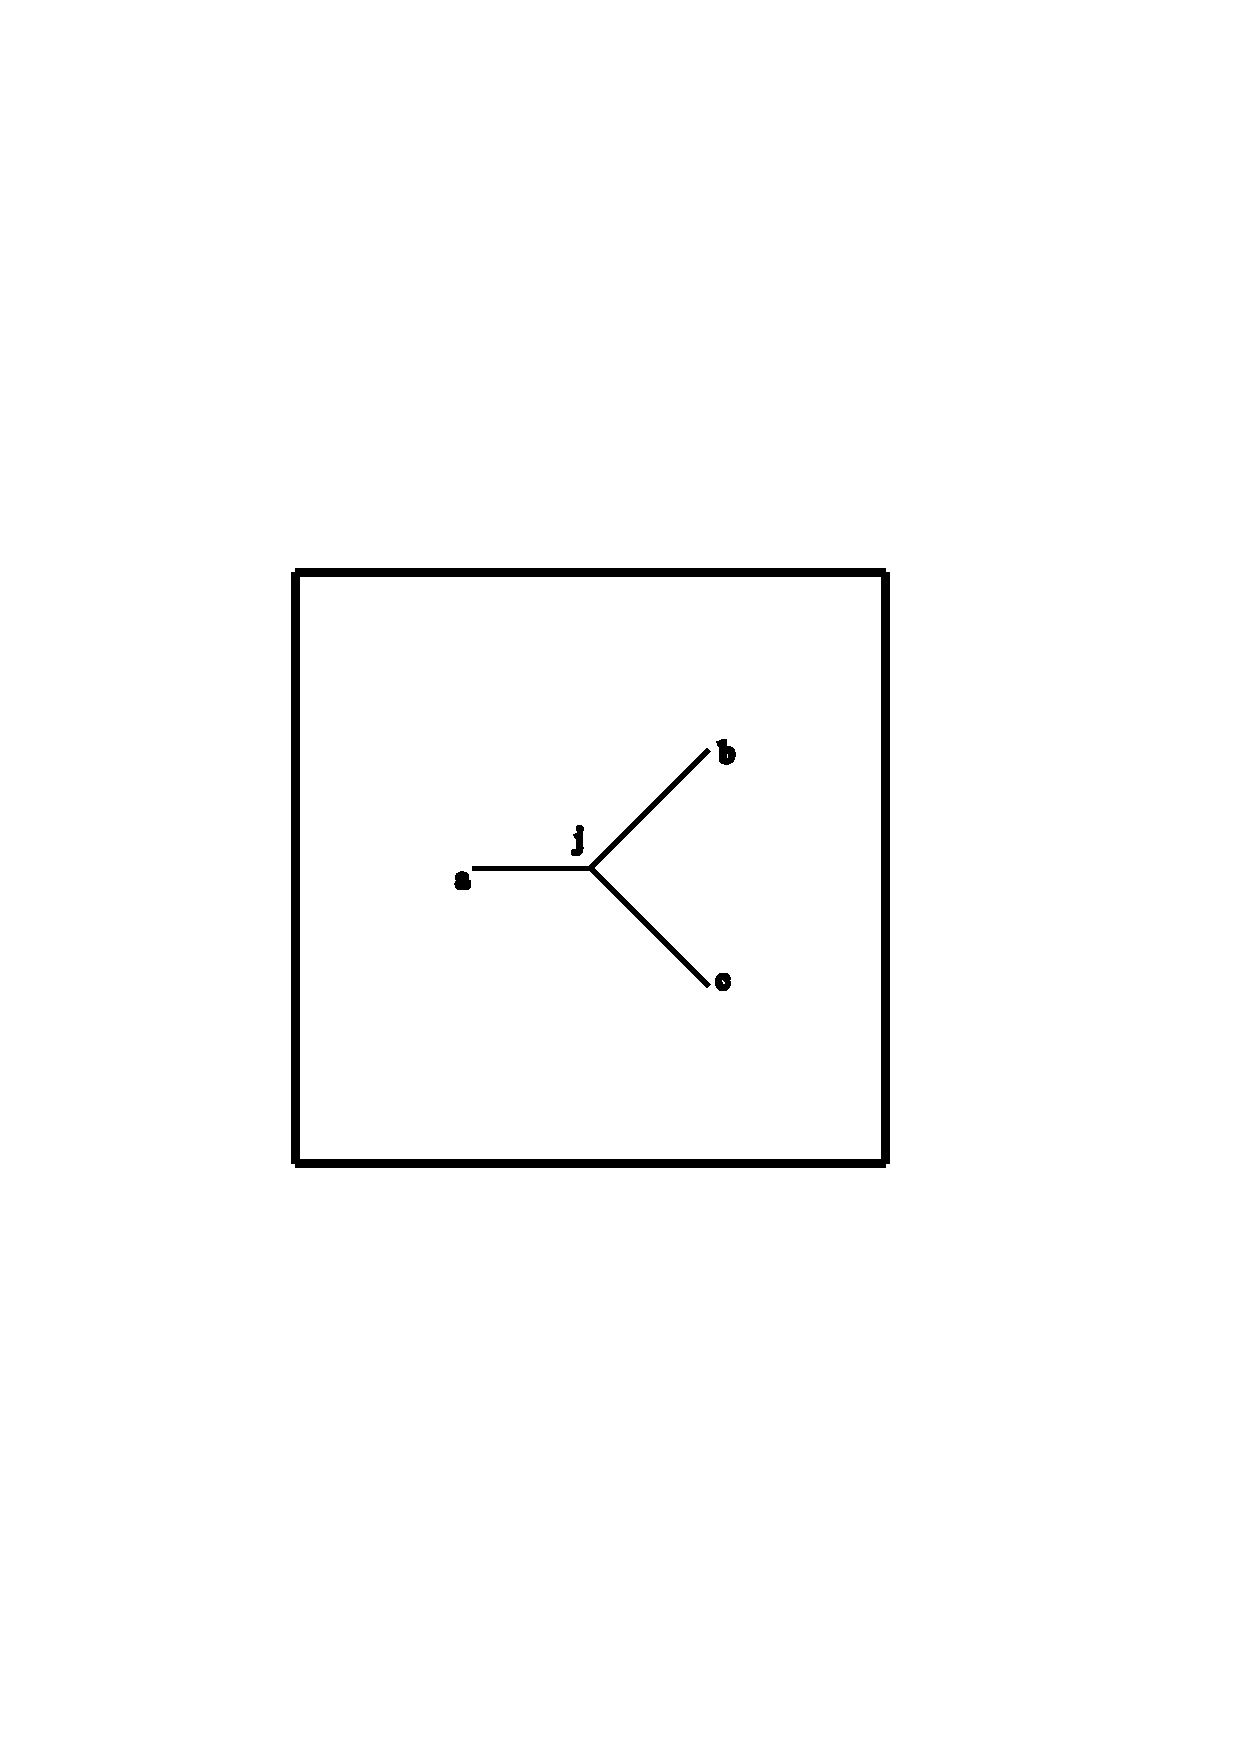
\includegraphics[width=0.3\textwidth]{FigtwoRight.pdf}
%			\end{figure}
%			%			\item \cite{ambrosio1990approximation} studied the relation between the phase field formulation and its sharp crack limit.
%		\end{itemize}
%		\item \textbf{Cons:}
%		\begin{itemize}
%			\item Need to track the complicated geometry of the evolving crack
%			\item Need extra input to predict complex phenomena
%		\end{itemize}
%	\end{itemize}
%\end{frame}

\begin{frame}[label=phasefield]
	\frametitle{Prelude: Smeared Crack Approaches}
	\framesubtitle{\SectionZero}
	%	\vspace{\baselineskip}
	\begin{itemize}
		\setlength\itemsep{2em}
		\item The phase field approaches to fracture
		\begin{itemize}
			\item Based on energy minimization with both displacement and crack path \cite{Francfort19981319}
			\item Use a \textbf{continuous} scalar field to denote the crack \cite{bourdin2008variational}
			\item Able to predict crack nucleation/branching without extra input
			\begin{figure}
				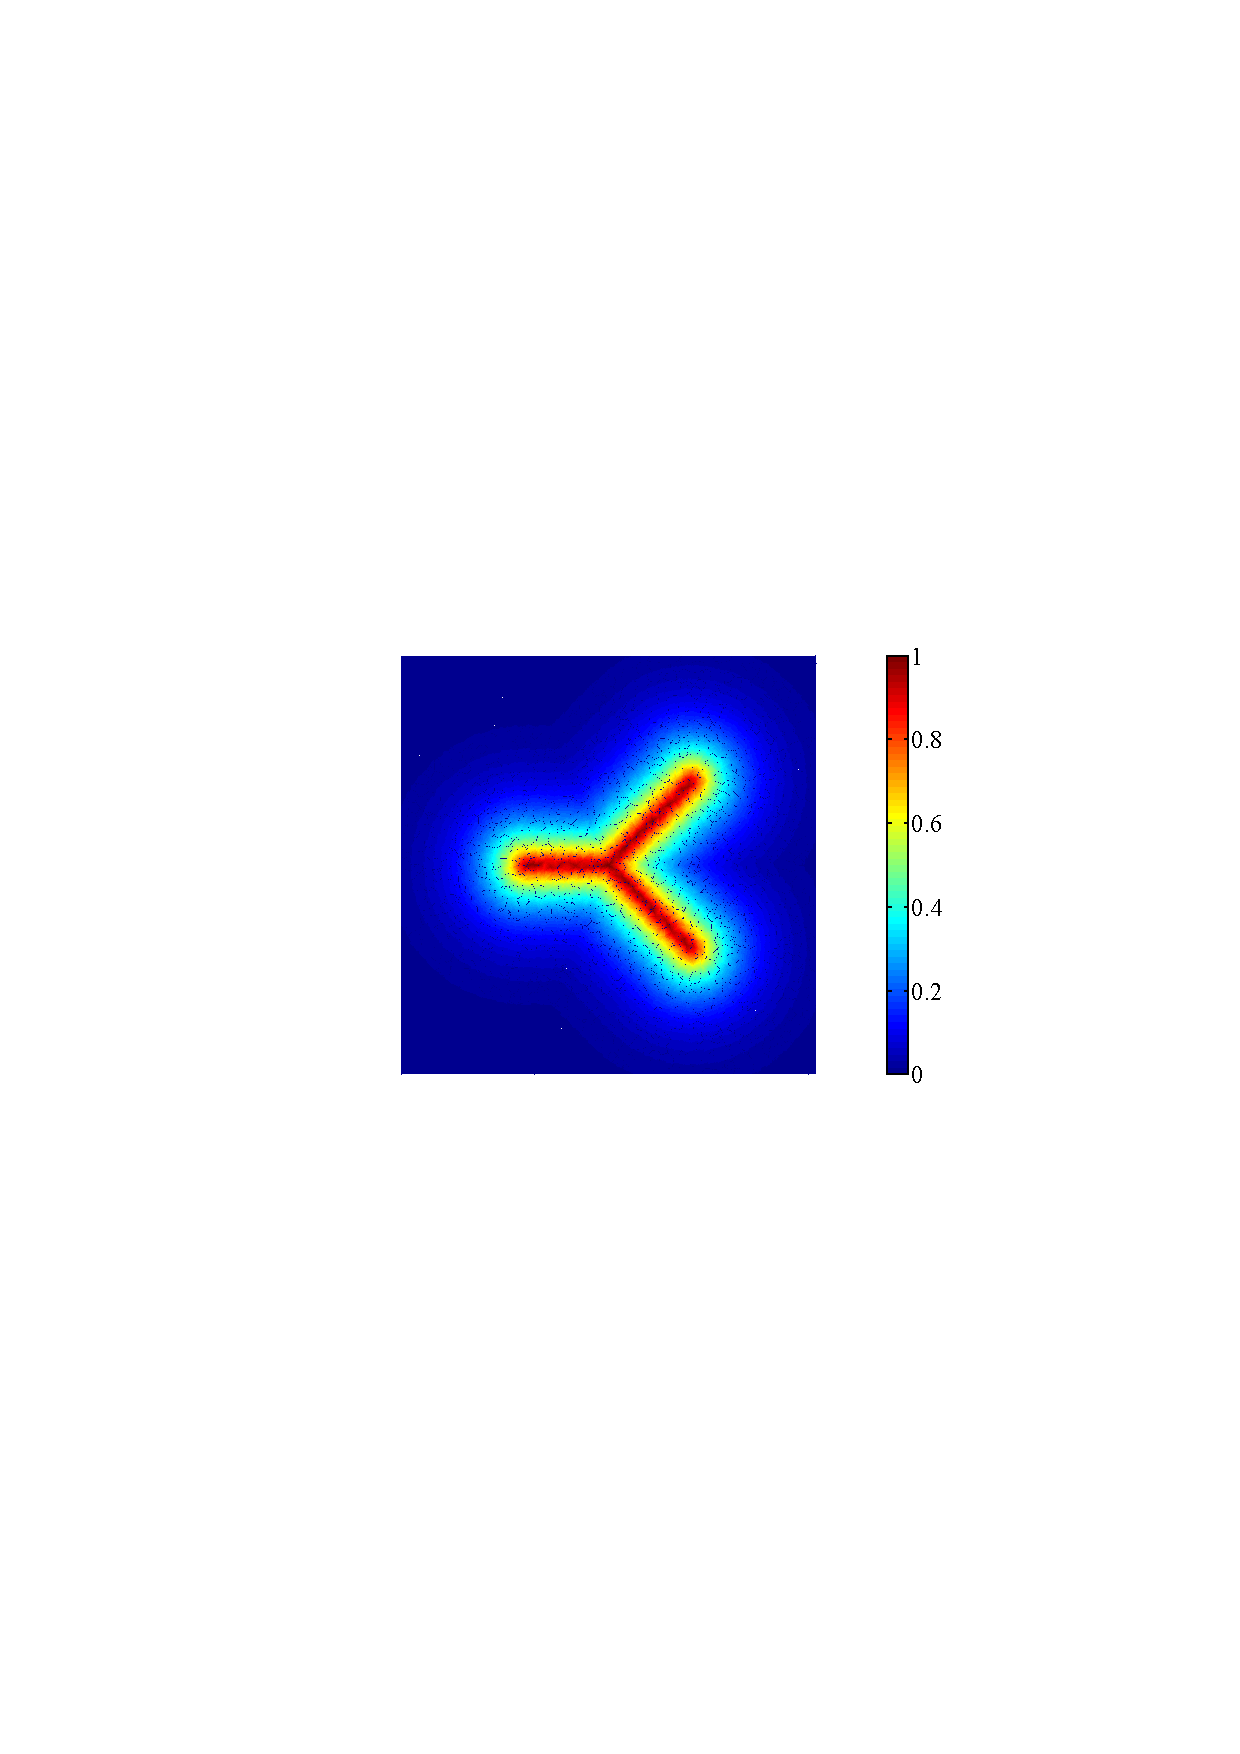
\includegraphics[width=0.4\textwidth]{colorbar.pdf}
			\end{figure}
			\item \textbf{Cons:}
			\begin{itemize}
				\item High computational cost
				\item Polyconvexity of the functional
			\end{itemize}
			%			\item \cite{ambrosio1990approximation} studied the relation between the phase field formulation and its sharp crack limit.
		\end{itemize}
	\end{itemize}
	\hyperlink{subexp}{\beamerbutton{supplemental}}
\end{frame}

%\begin{frame}
%	\frametitle{Outline}
%	%\framesubtitle{Massive parallelization and crack identification}
%	%	\vspace{\baselineskip}		
%	\begin{itemize}
%		\setlength\itemsep{2em}
%		\item \textbf{\SectionOne}
%		\item \textcolor{gray}{\SectionTwo}
%		\item \textcolor{gray}{\SectionThree}
%		\item \textcolor{gray}{\SectionFour}
%	\end{itemize}
%\end{frame}

\begin{frame}
	\frametitle{Outline}
	%\framesubtitle{Massive parallelization and crack identification}
	%	\vspace{\baselineskip}		
	\begin{itemize}
		\setlength\itemsep{2em}
		%\item \textcolor{gray}{\SectionOne}
		\item \textbf{\SectionTwo}
		\item \textcolor{gray}{\SectionThree}
		\item \textcolor{gray}{\SectionFour}
	\end{itemize}
\end{frame}

\begin{frame}
	\framesubtitle{\SectionTwo}
	\frametitle{Small Strain Measures}
	%	\vspace{\baselineskip}		
	\begin{itemize}
		\setlength\itemsep{2em}
		\item Let $\psi[\bm{\varepsilon}(\bm{u})]$ be the strain energy density which depends on the strain
		\begin{equation*}
		\label{aeq:4} \bm{\varepsilon}(\bm{u}) := 
		\frac{1}{2}\left(\nabla \bm{u}+\nabla \bm{u}^T\right)
		\end{equation*}
		as
		\begin{equation*}
		\psi(\bm{\varepsilon}) := \frac{\lambda}{2} (\trace\bm{\varepsilon})^2 + \mu \|\bm{\varepsilon}\|^2
		\end{equation*}
		\item Note that we exclude large strain measure, although most phenomenological models are based on hyperelastic formulation.
	\end{itemize}
	%\hyperlink{main}{\beamerbutton{main}}
\end{frame}

\begin{frame}
	\framesubtitle{\SectionTwo}
	\frametitle{Variational Formulation of Fracture}
	%	\vspace{\baselineskip}		
	\begin{itemize}
		\setlength\itemsep{2em}
%		\item For the case of an uncracked solid, the actual displacement is the minimizer of the following potential:
%		\begin{equation*}
%		E[\bm{u}] := \int_{\Omega}\psi[\bm{\varepsilon}(\bm{u})]\; d\Omega - \int_{\Omega}\bm{f}\cdot\bm{u} \; d\Omega -
%		\int_{\partial_N\Omega}\bm{t}_N\cdot \bm{u} \; d\Gamma
%		\end{equation*}
		\item The variational formulation for fracture of the solid consists in finding the minimizer of the following potential:
		\begin{equation*}
		\Pi[\bm{u}, \Gamma] := \int_{\Omega\setminus\Gamma}\psi[\bm{\varepsilon}(\bm{u})]\; d\Omega - \int_{\Omega}\bm{b}\cdot\bm{u} \; d\Omega -
		\int_{\partial_N\Omega}\bm{t}_N\cdot \bm{u} \; d\Gamma + g_c|\Gamma|
		\end{equation*}
		among all $\bm{u}:\mathbb{R}^2\rightarrow\mathbb{R}^2$ that are bounded deformation functions of $\Omega$ and that satisfy
		\begin{equation*}
			\bm{u} = \bm{u}_D, \quad \text{on~} \partial_D\Omega.
		\end{equation*}
		\item $\Gamma=\Gamma(\bm{u})\subset\Omega$ is the set of discontinuities of $\bm{u}$. $|\Gamma|$ denotes the length of $\Gamma$.
		\item But it is not easy to search among all possible $\Gamma$'s for minimization\ldots
%		\item The following Lagrangian is written for the brittle fracture of solids:
%		\begin{multline*}
%		L[\bm{u}, \dot{\bm{u}}] := \int_{\Omega\setminus\Gamma} \left\{\frac12 \rho \dot{\bm{u}}\cdot\dot{\bm{u}} - \psi_0[\bm{\varepsilon}(\bm{u})]\right\}\; d\Omega \\
%		+ \int_{\Gamma_N} \bm{t}_N\cdot \bm{u} \; d\Gamma + \int_{\Omega\setminus\Gamma}\rho \mathbf{b}\cdot\bm{u} \; d\Omega - g_c|\Gamma|
%		\end{multline*}
	\end{itemize}
\end{frame}
%
%
%\begin{frame}
%	\frametitle{Phase Field Approach}
%	
%	%	\vspace{\baselineskip}		
%	\begin{itemize}
%		\setlength\itemsep{2em}
%		\item Let:
%\begin{equation*}
%\begin{aligned}
%\mathscr{S}_u &:= \left\{\bm{u} \in H^1\left(\Omega; \mathbb{R}^2\right)\times[0,t_f] \middle|
%\bm{u}(\cdot,t) = \bm{u}_D(\cdot, t) \text{ on } \Gamma_D
%\right\}, \\
%\mathscr{S}_d &:= H^1(\Omega)\times[0,t_f].
%\end{aligned}
%\end{equation*}
%\item Find $(\bm{u}, d)\in\mathscr{S}_u\times\mathscr{S}_d$ that is the stationary point of the following functional:
%\begin{equation*}\label{RegVar}
%\begin{aligned}
%L_\ell[\bm{u}, \dot{\bm{u}}, d] := \int_\Omega \left\{\frac12 \rho \dot{\bm{u}}\cdot\dot{\bm{u}} - \psi[\bm{\varepsilon}(\bm{u}), d]\right\}\; d\Omega
%+ \int_{\Gamma_N} \bm{t}_N\cdot \bm{u} \; d\Gamma \\
% + \int_\Omega \rho \mathbf{b}\cdot\bm{u} \; d\Omega
%- \frac{g_c}{2}\int_\Omega \left(\frac{d^2}{\ell} + \ell \nabla d\cdot\nabla d\right)\;d\Omega
%\end{aligned}
%\end{equation*}
%	\end{itemize}
%\end{frame}

%\begin{frame}
%	\frametitle{\SectionOne}
%	\framesubtitle{Variational formulation of brittle fracture (to be regularized)}
%	%	\vspace{\baselineskip}		
%	\begin{itemize}
%		\setlength\itemsep{2em}
%		\item The variational formulation for the brittle fracture of the solid consists in finding the stationary point of the \textbf{action} $(S=\int_{0}^{t_f}L\; dt)$, following this Lagrangian: \cite{Francfort19981319}
%		\begin{multline*}
%		L[\bm{u}, \dot{\bm{u}}] := \underbrace{\int_{\Omega\setminus\Gamma} \left\{\frac12 \rho \dot{\bm{u}}\cdot\dot{\bm{u}} - \psi_0[\bm{\varepsilon}(\bm{u})]\right\}\; d\Omega}_{Kinetic~and~Elastic~Energies}\\
%		+ \underbrace{\int_{\Gamma_N} \bm{t}_N\cdot \bm{u} \; d\Gamma + \int_{\Omega\setminus\Gamma}\rho \mathbf{b}\cdot\bm{u} \; d\Omega}_{Work~by~External~Forces} - \underbrace{g_c|\Gamma|}_{Crack~Surface~Energy}
%		\end{multline*}
%		among all $\bm{u}:\mathbb{R}^2\times[0,t_f]\rightarrow\mathbb{R}^2$ that are bounded deformation functions of $\Omega$ and that satisfy
%		\begin{equation*}
%		\label{aeq:1}
%		\bm{u} = \bm{u}_D, \quad \text{on~} \Gamma_D\times[0,t_f].
%		\end{equation*}
%	\end{itemize}
%	%\hyperlink{supplemental}{\beamerbutton{supplemental}}
%\end{frame}
%

\begin{frame}
	\frametitle{Phase Field Regularization}
	\framesubtitle{\SectionTwo}
	%	\vspace{\baselineskip}		
	\begin{itemize}
		\setlength\itemsep{2em}
		\item We define a \textbf{continuous scalar field} ($d$) to denote the crack.
		\item We introduce the crack length functional, which takes the following form:
		\begin{equation*}%\label{Gamma}
		\begin{aligned}
		\Gamma_\ell[d]:=\int_\Omega\left(\frac{d^2}{2\ell} + \frac{\ell}{2}\nabla d\cdot\nabla d\right) d\Omega,
		\end{aligned}
		\end{equation*}
		where $\ell$ is a \textbf{length scale} such that when $\ell\rightarrow0$, the regularized formulation $\Gamma$-converges to that with explicit crack representation. \cite{Maso2005}
		\item $d:\Omega\rightarrow[0,1]$: In particular, regions with $d = 0$ and $d = 1$ correspond to ``perfect'' and ``fully-broken'' states of the material, respectively.
	\end{itemize}
\end{frame}

%
%\begin{frame}
%	\frametitle{\SectionOne}
%	\framesubtitle{Regularized variational formulation of brittle fracture (I)}
%	%	\vspace{\baselineskip}		
%	\begin{itemize}
%		\setlength\itemsep{2em}
%		\item One of the ingredients of the phase field approach is the \textbf{crack length functional}, which takes the following form:
%		\begin{equation*}
%		\Gamma_\ell[d]:=\frac12\int_\Omega\left(\frac{d^2}{\ell} + \ell \nabla d\cdot\nabla d\right) d\Omega,
%		\end{equation*}
%		where $\ell$ is a length scale such that when $\ell\rightarrow0$, the regularized formulation $\Gamma$-converges to that with explicit crack representation \cite{Maso2005}. 
%		\item $d:\Omega\rightarrow[0,1]$: In particular, regions with $d = 0$ and $d = 1$ correspond to perfect and fully broken states of the material, respectively.
%		% \item See Bourdin \emph{et al.} for the proof of the static anti-plane case.
%		%		\item The regularized variational formulation reads: Find $(\bm{u}, d)\in\mathscr{S}_u\times\mathscr{S}_d$ that is the stationary point of the following functional:
%		%		\begin{multline*}\label{RegVar}
%		%		L_l[\bm{u}, \dot{\bm{u}}, d] := \int_\Omega \left\{\frac12 \rho \dot{\bm{u}}\cdot\dot{\bm{u}} - \psi[\bm{\varepsilon}(\bm{u}), d]\right\}\; d\Omega \\
%		%		+ \int_{\Gamma_N} \bm{t}_N\cdot \bm{u} \; d\Gamma + \int_\Omega \rho \mathbf{b}\cdot\bm{u} \; d\Omega \\
%		%		- \frac{g_c}{2}\int_\Omega \left(\frac{d^2}{l} + l \nabla d\cdot\nabla d\right)\;d\Omega,
%		%		\end{multline*}
%	\end{itemize}
%\end{frame}
%
%\begin{frame}
%	\frametitle{\SectionOne}
%	\framesubtitle{Regularized variational formulation of brittle fracture (II)}
%	%	\vspace{\baselineskip}		
%	\begin{itemize}
%		\setlength\itemsep{2em}
%		\item Let 
%		\begin{equation*}
%		\begin{aligned}
%		\mathscr{S}_u &:= \left\{\bm{u} \in H^1\left(\Omega; \mathbb{R}^2\right)\times[0,t_f] \middle|
%		\bm{u}(\cdot,t) = \bm{u}_D(\cdot, t) \text{ on } \Gamma_D
%		\right\}, \\
%		\mathscr{S}_d &:= H^1(\Omega)\times[0,t_f].
%		\end{aligned}
%		\end{equation*}
%		\item The regularized variational formulation reads: Find $(\bm{u}, d)\in\mathscr{S}_u\times\mathscr{S}_d$ that is the stationary point of the action functional from the following Lagrangian:
%		\begin{multline*}\label{RegVar}
%		L_{\ell}[\bm{u}, \dot{\bm{u}}, d] := \int_\Omega \left\{\frac12 \rho \dot{\bm{u}}\cdot\dot{\bm{u}} - \psi[\bm{\varepsilon}(\bm{u}), d]\right\}\; d\Omega \\
%		+ \int_{\Gamma_N} \bm{t}_N\cdot \bm{u} \; d\Gamma + \int_\Omega \rho \mathbf{b}\cdot\bm{u} \; d\Omega \\
%		- \frac{g_c}{2}\int_\Omega \left(\frac{d^2}{\ell} + \ell\nabla d\cdot\nabla d\right)\;d\Omega.
%		\end{multline*}
%		%				\item Here $\psi(\bm{\varepsilon}, d)$ is the strain energy density degraded by the phase field such that
%		%				$\psi(\bm{\varepsilon}, 0) = \psi_0(\bm{\varepsilon})$ and that $\psi(\bm{\varepsilon}, d_1)\ge \psi(\bm{\varepsilon}, d_2)$ if $d_1<d_2$. 
%	\end{itemize}
%\end{frame}
%
%%\begin{frame}
%%	\frametitle{Phase Field Formulation with Time Adaptivity}
%%	\framesubtitle{Regularized variational formulation of brittle fracture}
%%	%	\vspace{\baselineskip}		
%%	\begin{itemize}
%%		\setlength\itemsep{2em}
%%		\item Here $\psi(\bm{\varepsilon}, d)$ is the strain energy density degraded by the phase field such that
%%		$\psi(\bm{\varepsilon}, 0) = \psi_0(\bm{\varepsilon})$ and that $\psi(\bm{\varepsilon}, d_1)\ge \psi(\bm{\varepsilon}, d_2)$ if $d_1<d_2$.
%%		\item The Euler-Lagrange equations read:
%%		\begin{subequations}
%%			\begin{align*}
%%			  -\rho\ddot{\bm{u}} + \divergence \bm{\sigma} + \rho \mathbf{b} &= \mathbf{0}, &\text{in~} \Omega\times[0,t_f], \\
%%			{-}\frac{\partial\psi}{\partial d} - \frac{g_c}{l}\left(d -  l^2 \Delta d\right) &= 0,  &\text{in~} \Omega\times[0,t_f], \\
%%			\bm{\sigma}\cdot\bm{n} - \bm{t}_N &= \bm{0}, &\text{on~} \partial_N\Omega\times[0,t_f], \\
%%			\frac{\partial d}{\partial \bm{n}} &= 0, &\text{on~} \partial \Omega\times[0,t_f],
%%			\end{align*}
%%		\end{subequations}
%%	\end{itemize}
%%\end{frame}
%
%\begin{frame}[label=mainweak]
%	\frametitle{\SectionOne}
%	\framesubtitle{Regularized variational formulation of brittle fracture (III)}
%	%	\vspace{\baselineskip}		
%	\begin{itemize}
%		\setlength\itemsep{2em}
%		\item Here $\psi(\bm{\varepsilon}, d)$ is the strain energy density degraded by the phase field such that
%		$\psi(\bm{\varepsilon}, 0) = \psi_0(\bm{\varepsilon})$ and that $\psi(\bm{\varepsilon}, d_1)\ge \psi(\bm{\varepsilon}, d_2)$ if $d_1<d_2$.
%		\item The Euler-Lagrange equations read:
%		\begin{subequations}
%			\begin{align*}
%			-\rho\ddot{\bm{u}} + \divergence \bm{\sigma} + \rho \mathbf{b} &= \mathbf{0}, &\text{in~} \Omega\times[0,t_f], \\
%			{-}\frac{\partial\psi}{\partial d} - \frac{g_c}{\ell}\left(d - {\ell}^2\Delta d\right) &= 0,  &\text{in~} \Omega\times[0,t_f], \\
%			\bm{\sigma}\cdot\bm{n} - \bm{t}_N &= \bm{0}, &\text{on~} \Gamma_N\times[0,t_f], \\
%			\frac{\partial d}{\partial \bm{n}} &= 0, &\text{on~} \partial\Omega\times[0,t_f],
%			\end{align*}
%		\end{subequations}
%		where $\bm{\sigma} = {\partial\psi}/{\partial\epsilon}$.
%	\end{itemize}
%	\hyperlink{suppweaki}{\beamerbutton{supplemental}}
%\end{frame}
%
%\begin{frame}
%	\frametitle{\SectionOne}
%	\framesubtitle{Three popular phase field models}
%	%	\vspace{\baselineskip}		
%	\begin{itemize}
%		\setlength\itemsep{2em}
%		\item What options are there for $\psi$?
%		\begin{itemize}
%			\item We recapitulate three popular phase field models.
%		\end{itemize}
%		\item These models mainly differ in the choice of the strain energy density $\psi(\bm{\varepsilon}, d)$,
%		for which we adopt the following general form:
%		\begin{equation*}\label{psi_general_form}
%		\psi(\bm{\varepsilon}, d)=(1-d)^2 \psi_+(\bm{\varepsilon}) + \psi_-(\bm{\varepsilon}),
%		\end{equation*}
%		where $\psi_+(\bm{\varepsilon})$ and $\psi_-(\bm{\varepsilon})$ are such that $\psi_+(\bm{\varepsilon}) + \psi_-(\bm{\varepsilon})=\psi_0(\bm{\varepsilon})$. 
%	\end{itemize}
%\end{frame}
%

\begin{frame}
	\framesubtitle{\SectionTwo}
	\frametitle{Regularized Variational Formulation of Fracture}
	%	\vspace{\baselineskip}		
	\begin{itemize}
		\setlength\itemsep{2em}
		\item We regularize the functional by means of the phase field:
		\begin{align*}
		&\Pi_\ell[\bm{u}, d] := \int_\Omega \psi[\bm{\varepsilon}(\bm{u}), d] \;d\Omega - \int_\Omega \mathbf{b}\cdot\bm{u} \; d\Omega - \int_{\partial_N\Omega} \bm{t}_N\cdot \bm{u} \; d\Gamma\\ 
		&+ {g_c}\int_\Omega \left(\frac{d^2}{2\ell} + \frac{\ell}{2} |\nabla d|^2\right)\;d\Omega.
		\end{align*}
		\item Here $\psi(\bm{\varepsilon}, d)$ is the strain energy density degraded by the phase field such that
		$\psi(\bm{\varepsilon}, 0) = \psi_0(\bm{\varepsilon})$ and that $\psi(\bm{\varepsilon}, d_1)\ge \psi(\bm{\varepsilon}, d_2)$ if $d_1<d_2$.
%		\item Let $\psi(\bm{\varepsilon}, d) = g(d)\psi_0$. Let $g(d)=(1-d)^2$. Hence, $g(0) = 1$, $g(1) = 0$, and $g\prime = 1$ 
		\item Now we look for various ways to degrade the strain energy density\ldots
	\end{itemize}
\end{frame}

\begin{frame}
	\framesubtitle{\SectionTwo}
	\frametitle{Popular Phase Field Models (A)}
	%	\vspace{\baselineskip}		
	\begin{itemize}
		\setlength\itemsep{2em}
		\item \textbf{Model A:} This is the original model proposed for similar formulations. It is convenient in that $\psi$ is analytic in both $d$ and $\bm{\varepsilon}$. \cite{bourdin2008variational}
		\begin{align*}
		\psi&=(1-d)^2\psi_{+} + \psi_{-},\quad\sigma=\frac{\partial\psi}{\partial\varepsilon}, \\
		\psi_+&=\frac{\lambda}{2} (\trace\bm{\varepsilon})^2 + \mu \|\bm{\varepsilon}\|^2,\\
		\psi_-&=0.
		%		\partial\psi_+/\partial\bm{\varepsilon}=\lambda(\trace\bm{\varepsilon})\bm{1} + 2\mu\bm{\varepsilon},\quad\partial\psi_-/\partial\bm{\varepsilon}=0.
		\end{align*}
		%		And:
		%		\begin{equation*}
		%		\bm{\sigma}(\bm{\varepsilon}, d) = \frac{\partial\psi}{\partial \bm{\varepsilon}} = (1-d)^2 \frac{\partial\psi_+}{\partial \bm{\varepsilon}}
		%		\end{equation*}	
	\end{itemize}
\end{frame}

\begin{frame}
	\framesubtitle{\SectionTwo}
	\frametitle{Popular Phase Field Models (B)}
	%	\vspace{\baselineskip}		
	\begin{itemize}
		\setlength\itemsep{2em}
		\item \textbf{Model B:} This model assumes that both volumetric expansion and deviatoric deformation contribute to crack propagation but not volumetric compression. \cite{Amor09}
		\begin{align*}
		\psi&=(1-d)^2\psi_{+} + \psi_{-},\quad\sigma=\frac{\partial\psi}{\partial\varepsilon}, \\
		\psi_+&=(\lambda+2\mu/3)\langle \trace \bm{\varepsilon} \rangle_+\bm{1} + 2\mu\dev\bm{\varepsilon},\\
		\psi_-&=(\lambda+2\mu/3)\langle \trace \bm{\varepsilon} \rangle_-\bm{1}.
		\end{align*}
		%		And:
		%		\begin{equation*}
		%		\bm{\sigma}(\bm{\varepsilon}, d) = \frac{\partial\psi}{\partial \bm{\varepsilon}} = (1-d)^2 \frac{\partial\psi_+}{\partial \bm{\varepsilon}} + \frac{\partial\psi_-}{\partial \bm{\varepsilon}}
		%		\end{equation*}
	\end{itemize}
\end{frame}

\begin{frame}
	\framesubtitle{\SectionTwo}
	\frametitle{Popular Phase Field Models (C)}
	%	\vspace{\baselineskip}		
	\begin{itemize}
		\setlength\itemsep{2em}
		\item \textbf{Model C:} This model postulates that the stress degradation is due to a combination of tensile loading and volumetric expansion. \cite{Miehe10}
		%		\begin{equation*}
		%		\bm{\sigma}(\bm{\varepsilon}, d) = \frac{\partial\psi}{\partial \bm{\varepsilon}} = (1-d)^2 \frac{\partial\psi_+}{\partial \bm{\varepsilon}} + \frac{\partial\psi_-}{\partial \bm{\varepsilon}}
		%		\end{equation*}
		%		where
		\begin{align*}
		\psi&=(1-d)^2\psi_{+} + \psi_{-},\quad\sigma=\frac{\partial\psi}{\partial\varepsilon}, \\
		\psi_+&=\lambda \langle \trace \bm{\varepsilon} \rangle_+ \bm{1} + 2\mu \sum_{i=1}^3 \langle\varepsilon_i\rangle_+\mathbf{n}_i\otimes\mathbf{n}_i, \\
		\psi_-&=\lambda \langle \trace \bm{\varepsilon} \rangle_- \bm{1} + 2\mu \sum_{i=1}^3 \langle\varepsilon_i\rangle_-\mathbf{n}_i\otimes\mathbf{n}_i.
		\end{align*}
	\end{itemize}
\end{frame}

%\begin{frame}
%	\frametitle{\SectionOne}
%	\framesubtitle{Variational formulation of brittle fracture (to be regularized)}
%	%	\vspace{\baselineskip}		
%	\begin{itemize}
%		\setlength\itemsep{2em}
%		\item $\psi_0[\bm{\varepsilon}(\bm{u})]$ the strain energy density which depends on the strain
%		\begin{equation*}
%		\label{aeq:4} \bm{\varepsilon}(\bm{u}) := 
%		\frac{1}{2}\left(\nabla \bm{u}+\nabla \bm{u}^T\right)
%		\end{equation*}
%		as
%		\begin{equation*}
%		\psi_0(\bm{\varepsilon}) := \frac{\lambda}{2} (\trace\bm{\varepsilon})^2 + \mu \|\bm{\varepsilon}\|^2
%		\end{equation*}
%		\item $\Gamma=\Gamma(\bm{u})\subset\Omega$ is the set of discontinuities of $\bm{u}(\cdot, t)$ such that the irreversibility of the crack is satisfied. $|\Gamma|$ denotes the length of $\Gamma$.
%		\item But it is not easy to search among all possible $\Gamma$'s for minimization\ldots
%	\end{itemize}
%	%\hyperlink{main}{\beamerbutton{main}}
%\end{frame}

%\begin{frame}[label=staticweak]
%	\frametitle{\SectionTwo}
%	\framesubtitle{The first variation}
%	%	\vspace{\baselineskip}		
%	\begin{itemize}
%		\setlength\itemsep{2em}
%		\item Taking the first variation yield:
%		\begin{multline*}
%			\delta \Pi_\ell[(\bm{u}, d), (\bm{w}, q)] :=  \left.\frac{d}{d\epsilon} \Pi_\ell[\bm{u} + \epsilon\bm{w}, d + \epsilon q]\right|_{\epsilon=0} \\
%			=\int_\Omega \bm{\sigma}[\bm{\varepsilon}(\bm{u}), d] : \bm{\varepsilon}(\bm{w}) \;d\Omega - \int_{\Gamma_N} \bm{t}_N\cdot \bm{w} \; d\Gamma - \int_\Omega \mathbf{b}\cdot\bm{w} \; d\Omega \\
%			\quad - \int_\Omega 2(1-d) q \psi_+(\bm{\varepsilon}) \; d\Omega + 
%			g_c\int_\Omega\left(\frac{d\;q}{\ell} + \ell \nabla d\cdot\nabla q\right)\;d\Omega
%		\end{multline*}
%		where 
%		\begin{equation*}
%		\bm{\sigma}:=\frac{\partial\psi}{\partial\bm{\varepsilon}} = \left[(1-d)^2 + k\right] \frac{\partial\psi_+(\bm{\varepsilon})}{\partial\bm{\varepsilon}} + \frac{\partial\psi_-(\bm{\varepsilon})}{\partial\bm{\varepsilon}}
%		\end{equation*}
%		is the Cauchy stress tensor.
%	\end{itemize}
%\end{frame}

%\begin{frame}[label=staticweak]
%	\framesubtitle{\SectionTwo}
%	\frametitle{The Weak Form}
%	%	\vspace{\baselineskip}		
%	\begin{itemize}
%		\setlength\itemsep{2em}
%		\item Find $(\bm{u}, d) \in H^1(\Omega; \mathbb{R}^2)\times H^1(\Omega)$ with $\bm{u}=\bm{u}_D$ on $\partial_D\Omega$, such that for all $(\bm{w}, q) \in H^1(\Omega; \mathbb{R}^2)\times H^1(\Omega)$ with $\bm{w}=\bm{0}$ on $\partial_D\Omega$, $\delta \Pi_\ell[(\bm{u}, d), (\bm{w}, q)]=0$, or equivalently:
%		\begin{align*}
%		&\int_\Omega \bm{\sigma}[\bm{\varepsilon}(\bm{u}), d] : \bm{\varepsilon}(\bm{w}) \;d\Omega = \int_\Omega \mathbf{b}\cdot\bm{w} \; d\Omega + \int_{\partial_N\Omega} \bm{t}_N\cdot \bm{w} \; d\Gamma, \\
%		&\int_\Omega \left[2d q \psi_+(\bm{\varepsilon})+g_c\left(\frac{d\;q}{\ell} + \ell \nabla d\cdot\nabla q\right)\right]\;d\Omega =
%		\int_\Omega 2q \psi_+(\bm{\varepsilon}) \;d\Omega.
%		\end{align*}
%	\end{itemize}
%	\hyperlink{subfstvar}{\beamerbutton{supplemental}}
%\end{frame}
%
%\begin{frame}
%	\framesubtitle{\SectionTwo}
%	\frametitle{The Tangent Stiffness Matrices}
%	%	\vspace{\baselineskip}		
%	\begin{itemize}
%		\setlength\itemsep{2em}
%		\item We normally solve for the phase field formulation with iterations between the elasticity half problem and the phase field half problem.
%		\item The tangent stiffness matrices are then given by:
%		\begin{align*}
%		K_{PQ} &= \int_\Omega \bm{\varepsilon}(\mathbf{N}_P): \mathbb{A}[\bm{\varepsilon}(\bm{u}), d] : \bm{\varepsilon}(\mathbf{N}_Q)  \;d\Omega, \\
%		\overline{K}_{PQ} &= \int_\Omega 2 \phi_P \psi_+(\bm{\varepsilon}) \phi_Q \; d\Omega + 
%		g_c\int_\Omega  \left[\frac{\phi_P \phi_Q}{\ell} + \ell \nabla \phi_P \cdot \nabla \phi_Q \right]\;d\Omega
%		\end{align*}
%		where the fourth-order tensor
%		\begin{equation*}
%		\mathbb{A}[\bm{\varepsilon}(\bm{u}), d] := \left.\frac{\partial \bm{\sigma}(\bm{\varepsilon}, d)}{\partial \bm{\varepsilon}}\right|_{\bm{\varepsilon}=\bm{\varepsilon}(\bm{u})}
%		\end{equation*}
%		is the tangent elastic modulus tensor.
%	\end{itemize}
%\end{frame}

\begin{frame}
	\frametitle{Outline}
	%\framesubtitle{Massive parallelization and crack identification}
	%	\vspace{\baselineskip}		
	\begin{itemize}
		\setlength\itemsep{2em}
		%\item \textcolor{gray}{\SectionOne}
		\item \textcolor{gray}{\SectionTwo}
		\item \textbf{\SectionThree}
		\item \textcolor{gray}{\SectionFour}
	\end{itemize}
\end{frame}

\begin{frame}[label=RegVarInc]
	\framesubtitle{\SectionThree}
	\frametitle{Regularized Variational Formulation of Fracture}
	%	\vspace{\baselineskip}		
	\begin{itemize}
		\setlength\itemsep{2em}
		\item Let
		\begin{equation*}
				\begin{aligned}
				\mathscr{S}_u &:= \left\{\bm{u} \in H^1\left(\Omega; \mathbb{R}^2\right)\middle|
				\bm{u}(\cdot) = \bm{u}_D(\cdot) \text{ on } \partial_D\Omega
				\right\},\\
			\mathscr{S}_p &:= L^2(\Omega),\\
				\mathscr{S}_d &:= H^1(\Omega).
				\end{aligned}
		\end{equation*}
		\item We aim to minimize the following potential: \cite{Wheeler201469}
				\begin{equation*}
				\begin{aligned}
				&\Pi_\ell[\bm{u},p,d] := \int_\Omega \psi^{Dev}[\bm{\varepsilon}(\bm{u}), d] \;d\Omega +
				\int_\Omega \left({-}\frac{p^2}{2\lambda}+p\divergence\bm{u}\right) \;d\Omega\\
				&- \int_{\partial_N\Omega} \bm{t}_N\cdot \bm{u} \; d\Gamma - \int_\Omega \rho\mathbf{b}\cdot\bm{u} \; d\Omega + {g_c}\int_\Omega \left(\frac{d^2}{2\ell} + \frac{\ell}{2} |\nabla d|^2\right)\;d\Omega.
				\end{aligned}
				\end{equation*}				
	\end{itemize}
	\hyperlink{subinc}{\beamerbutton{supplemental}}
\end{frame}

\begin{frame}
	\framesubtitle{\SectionThree}
	\frametitle{The Strong Form}
	%	\vspace{\baselineskip}		
	\begin{itemize}
		\setlength\itemsep{2em}
%		\item Find $(\bm{u}, d) \in H^1(\Omega; \mathbb{R}^2)\times H^1(\Omega)$ with $\bm{u}=\bm{u}_D$ on $\Gamma_D$, such that for all $(\bm{w}, q) \in H^1(\Omega; \mathbb{R}^2)\times H^1(\Omega)$ with $\bm{w}=\bm{0}$ on $\Gamma_D$, $\delta \Pi_\ell[(\bm{u}, d), (\bm{w}, q)]=0$, or equivalently:

%		\item Let $(\bm{u},p,d)\in H^1(\Omega;\mathbb{R}^2)\times L^2(\Omega)\times H^1(\Omega)$ with $\bm{u}=\bm{u}_D$ on $\Gamma_D$.
		
%		\begin{equation*}
%		\begin{aligned}
%		\mathscr{S}_u &:= \left\{\bm{u} \in H^1\left(\Omega; \mathbb{R}^2\right)\middle|
%		\bm{u}(\cdot) = \bm{u}_D(\cdot) \text{ on } \Gamma_D
%		\right\},\\
%		\mathscr{S}_d &:= H^1(\Omega),\\
%		\mathscr{S}_p &:= L^2(\Omega).
%		\end{aligned}
%		\end{equation*}
		\item The Euler-Lagrange equations read:
		\begin{subequations}
			\begin{align*}
			\divergence \bm{\sigma}^{Dev} + \nabla p + \mathbf{b} &= \mathbf{0}, &\text{in~}\Omega,\\
			\left({-}\frac{1}{\lambda}p+\divergence\bm{u}\right) &= 0,&\text{in~}\Omega,\\
			{-}\frac{\partial{\psi}^{Dev}}{\partial d} - \frac{g_c}{\ell}\left(d - {\ell}^2\Delta d\right) &= 0,  &\text{in~} \Omega, \\
			\left(\bm{\sigma}^{Dev}\cdot\bm{n}\right) - \bm{t}_N &= \bm{0}, &\text{on~} \partial_N\Omega,\\	
			%p &= 0, &\text{on~} \partial\Omega, \\
			\frac{\partial d}{\partial \bm{n}} &= 0, &\text{on~} \partial\Omega,\\
			\bm{u} &= \bm{u}_D, &\text{on~} \partial_D\Omega.
%			\frac{\partial p}{\partial \bm{n}} &= 0, &\text{on~} \partial\Omega.
%			\nabla p\cdot\bm{n} &= 0, &\text{on~} \partial\Omega.
			\end{align*}
		\end{subequations}
	\end{itemize}
\end{frame}

\begin{frame}
	\framesubtitle{\SectionThree}
	\frametitle{The Weak Form}
	%	\vspace{\baselineskip}		
	\begin{itemize}
		\setlength\itemsep{2em}
%		\item To proceed, we let the test function spaces be
%		\begin{equation*}
%		\begin{aligned}
%		\mathscr{V}_u &:= \left\{\bm{w}\in H^1\left(\Omega; \mathbb{R}^2\right) \middle|
%		\bm{w} = \mathbf{0} \text{ on } \Gamma_D
%		\right\},\quad
%		\mathscr{V}_p := L^2(\Omega),\mathscr{V}_d := H^1(\Omega).
%		\end{aligned}
%		\end{equation*}
		\item The weak form can be stated as: Find $(\bm{u},p,d)\in\mathscr{S}_u\times\mathscr{S}_p\times\mathscr{S}_d$ such that for all $\bm{w}\in\mathscr{V}_u$, $\tilde{p}\in\mathscr{V}_p$, and $q\in \mathscr{V}_d$:
		\begin{subequations}
		\begin{align*}
		&\int_\Omega \bm{\sigma}^{Dev}[\bm{\varepsilon}(\bm{u}), d] : \bm{\varepsilon}^{Dev}(\bm{w}) \;d\Omega + \int_\Omega p\divergence\bm{w} \;d\Omega\\
		&= \int_{\partial_N\Omega} \bm{t}_N\cdot \bm{w} \; d\Gamma + \int_\Omega \mathbf{b}\cdot\bm{w} \; d\Omega,\\
		&\int_{\Omega} \left({-}\frac{1}{\lambda}p+\divergence\bm{u}\right)\tilde{p}\; d\Omega=0,\\
		&\int_\Omega \left[2d q \psi^{Dev}_+(\bm{\varepsilon})+g_c\left(\frac{d\;q}{\ell} + \ell \nabla d\cdot\nabla q\right)\right]\;d\Omega =
		\int_\Omega 2q \psi^{Dev}_+(\bm{\varepsilon}) \;d\Omega.
		\end{align*}			
		\end{subequations}
	\end{itemize}
\end{frame}

\begin{frame}
	\frametitle{Outline}
	%\framesubtitle{Massive parallelization and crack identification}
	%	\vspace{\baselineskip}		
	\begin{itemize}
		\setlength\itemsep{2em}
		\item \textcolor{gray}{\SectionOne}
		\item \textcolor{gray}{\SectionTwo}
		\item \textcolor{gray}{\SectionThree}
		\item \textbf{\SectionFour}
	\end{itemize}
\end{frame}

\begin{frame}[fragile, label=fenics]
	\frametitle{\SectionFour}
	\framesubtitle{Features}
	%	\vspace{\baselineskip}
	%\newcommand\codeHighlight[1]{\textcolor[rgb]{1,0,0}{\textbf{#1}}}
	%		\item \textbf{PETSc} is a suite of data structures and routines for the solution of partial differential equations.
	\begin{itemize}
		\setlength\itemsep{2em}
		\item The \textbf{FEniCS Project} is a collection of free software with an extensive list of features for efficient solution of differential equations. \\
\newcommand\codeHighlight[1]{\textcolor[rgb]{1,0,0}{\textbf{#1}}}
\begin{Verbatim}[commandchars=\\\{\}]
energy_elastic = psi(epsdev(u_), d_) * dx
...
Residual_u = \codeHighlight{derivative} (energy_total, v_, v_t)
Jacobian_u = \codeHighlight{derivative} (Residual_u, v_, v)
\end{Verbatim}		
		\item We use the FEniCS project and PETSc software packages:
		\begin{itemize}
			\item ``Rigid Punch Incompressible Elasticity'' by \textbf{Jack~S.~Hale}
			\item ``FEniCS Variational Damage and Fracture'' by \textbf{Corrado~Maurini}
			\textit{Available online at {\color{blue}{\href{url}{https://bitbucket.org/cmaurini/~}}}}
			\item ``Phase Field Models with Incompressibility'' by \textbf{Vahid~Ziaei-Rad}
		\end{itemize}
	\end{itemize}
	\hyperlink{subfstvarii}{\beamerbutton{supplemental}}
\end{frame}

%\begin{frame}
%	\frametitle{\SectionFour}
%	\framesubtitle{Cracked square plate under a tension test: Without incompressibility}
%		\vspace{\baselineskip}		
%	\begin{itemize}
%		\item Mobel by \cite{Amor09}
%%		\setlength\itemsep{2em}
%%		\begin{center}
%%			\includemedia[
%%			activate=onclick,
%%			width=0.5\textwidth
%%			]{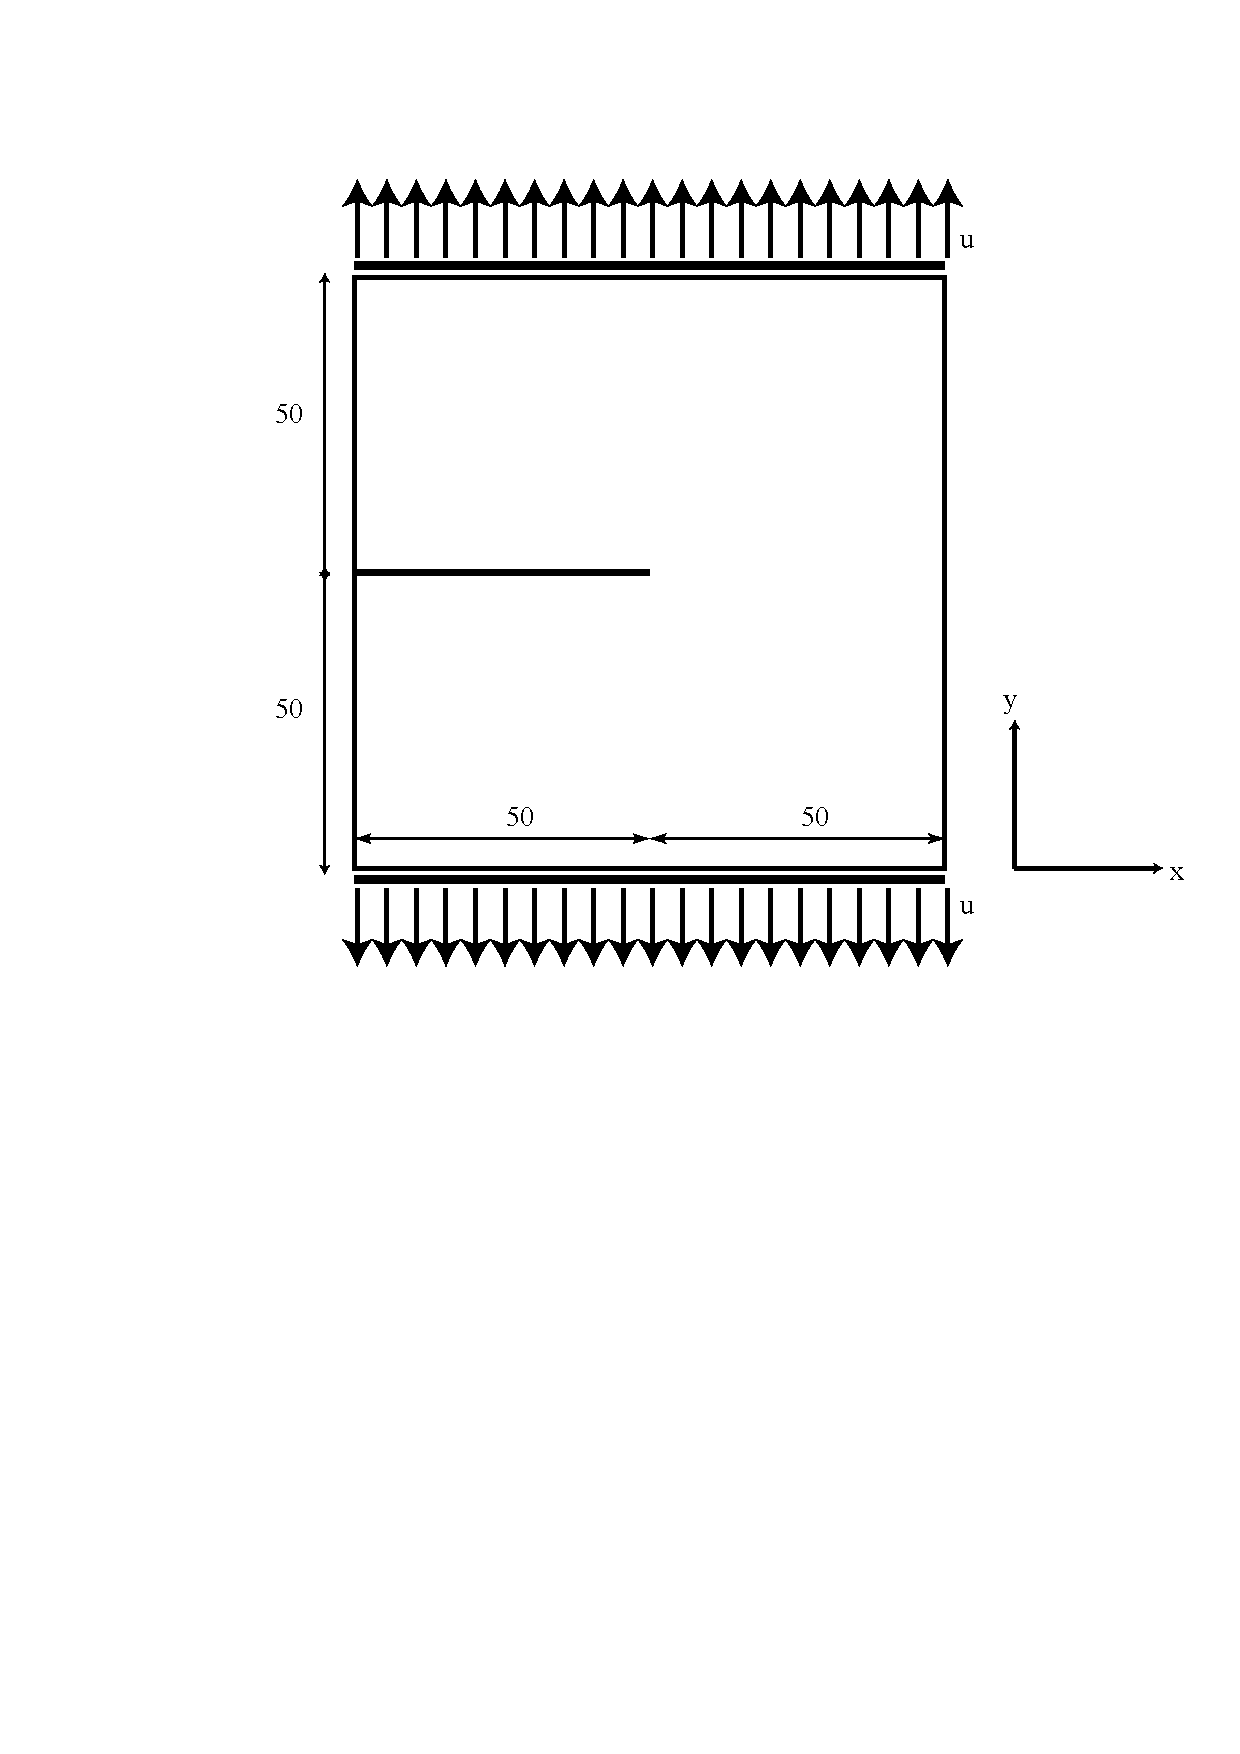
\includegraphics{./Sample-setup.pdf}}{./Tension_B_Amor_Low.swf}
%%		\end{center}
%		\begin{center}
%		\includemedia[activate=onclick,
%		width=0.5\textwidth
%		]{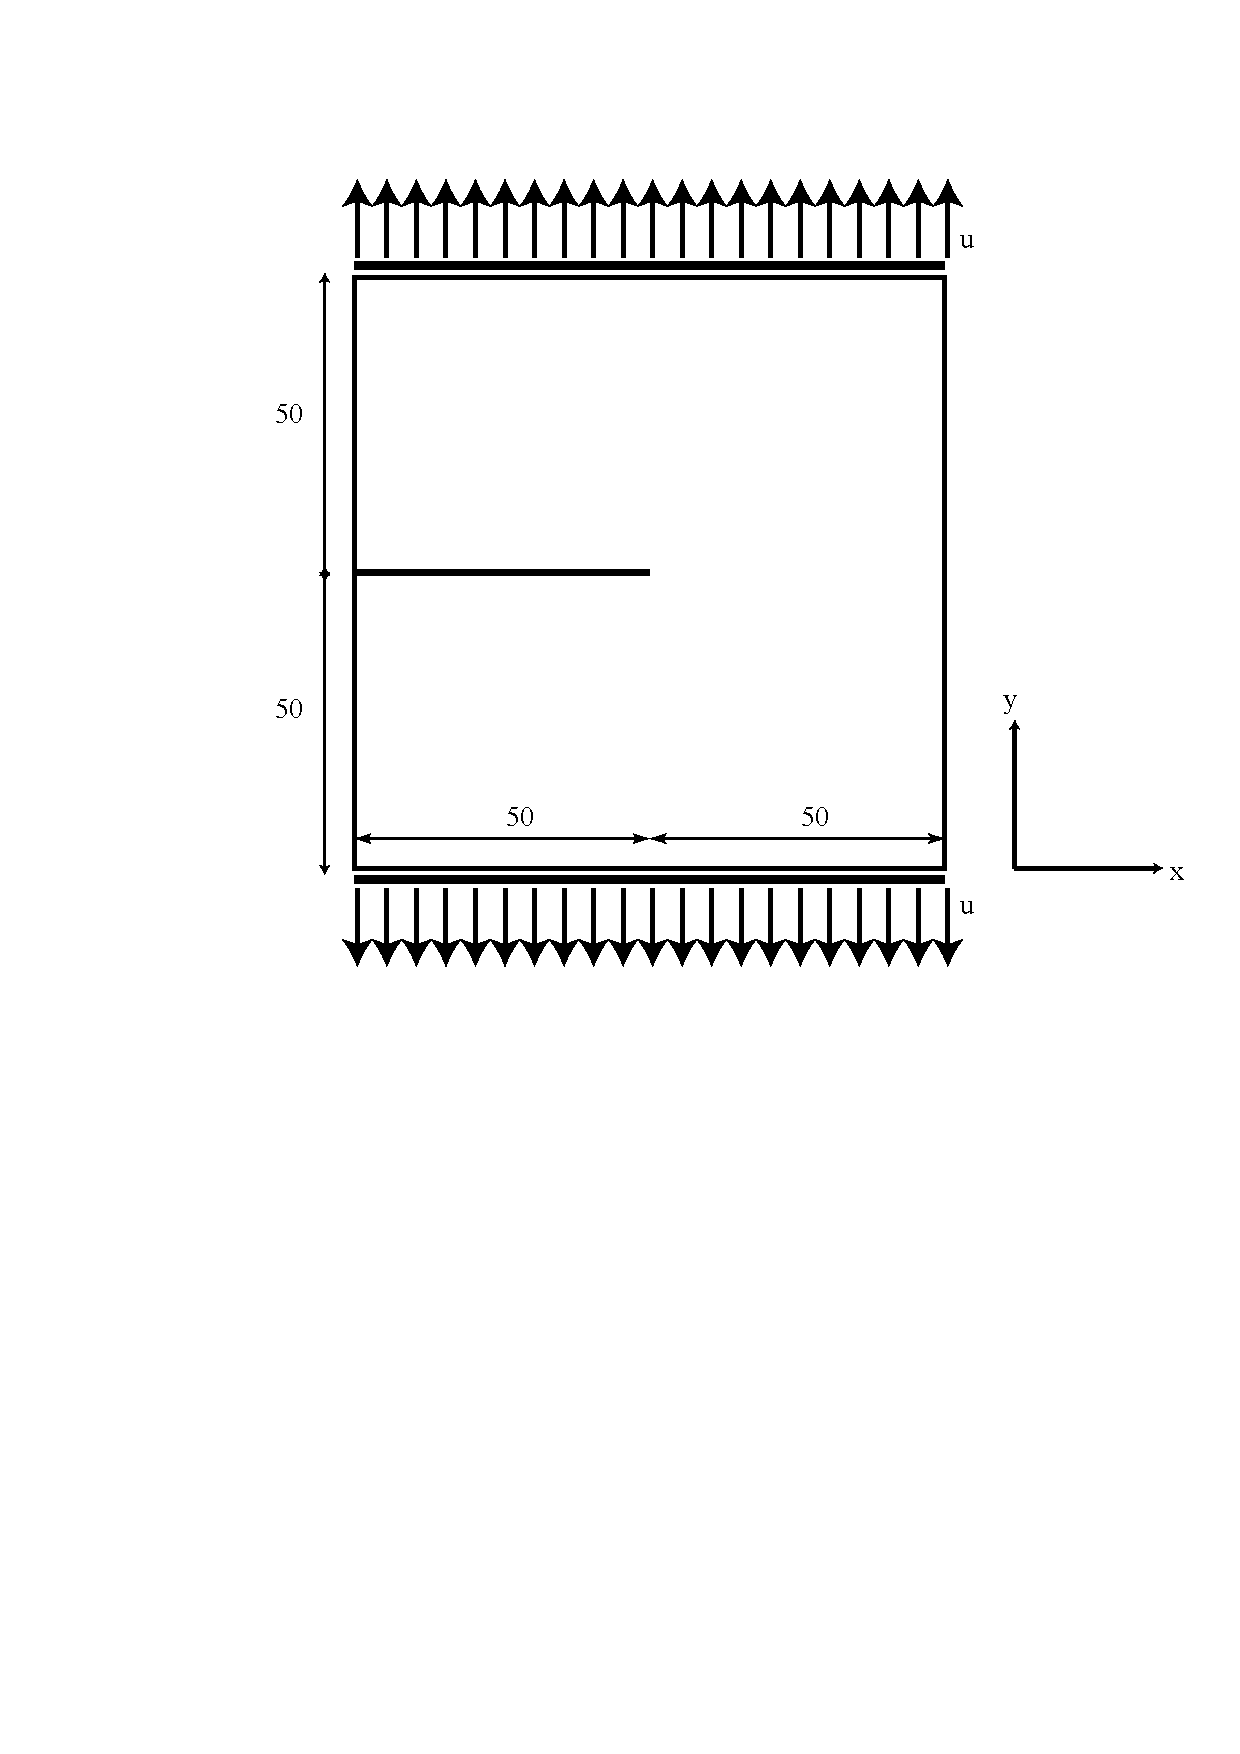
\includegraphics{Sample-setup.pdf}}{./Tension_B_Amor_Low.swf}
%		\end{center}
%	\end{itemize}
%\end{frame}

%\begin{frame}
%	\frametitle{\SectionTwo}
%
%%	\vspace{\baselineskip}		
%	\begin{itemize}
%		\setlength\itemsep{2em}
%			\item Consider a one-dimensional \emph{Lagrangian} system:
%			\begin{equation*}
%			L(\bm{u},\dot{\bm{u}})=\frac12 m\dot{\bm{u}}^2-\frac12 k\bm{u}^2
%			\end{equation*}
%			\item We form the \emph{action} functional by integrating $L$ over the time domain:
%			\begin{equation*}
%			S(\bm{u},\dot{\bm{u}})=\int_{0}^{T} L\left(\bm{u}(t),\dot{\bm{u}}(t)\right)\; dt
%			\end{equation*}
%			\item We compute \emph{variations of action} to find the trajectory of motion:
%			\begin{equation*}
%				\delta S(\bm{u},\dot{\bm{u}})= 0
%			\end{equation*}
%	\end{itemize}
%\end{frame}
%
%\begin{frame}
%	\frametitle{\SectionTwo}
%	
%	%	\vspace{\baselineskip}		
%	\begin{itemize}
%		\setlength\itemsep{2em}
%		\item The Euler-Lagrange equation of motion is given by:
%		\begin{equation*}
%		\frac{\partial L(\bm{u},\dot{\bm{u}})}{\partial \bm{u}} - 
%		\frac{d}{dt}\left(\frac{\partial L(\bm{u},\dot{\bm{u}})}{\partial \dot{\bm{u}}}\right) = 0
%		\end{equation*}
%		\item For the particular form of Lagrangian chose, this is just \textbf{Newton's second law}:
%		\begin{equation*}
%		m\ddot{\bm{u}}=-k\bm{u}
%		\end{equation*}
%	\end{itemize}
%\end{frame}
%
%\begin{frame}
%	\frametitle{\SectionTwo}
%	
%	%	\vspace{\baselineskip}		
%	\begin{itemize}
%		\setlength\itemsep{2em}
%		\item The idea is to discretize the \emph{variational principle} rather than the differential equations.
%		\item Let $L_d$ be an approximation to the action functional:
%		\begin{equation*}
%		L_d(\bm{u}^k, \bm{u}^{k+1})\simeq\int_{t_k}^{t_{k+1}}L\left(\bm{u},\dot{\bm{u}}\right)\; dt
%		\end{equation*}
%		\item A simple example might be:
%		\begin{equation*}
%		L_d(\bm{u}^k,\bm{u}^{k+1},\Delta t)=\Delta t\left[\left({\frac{\bm{u}^{k+1}-\bm{u}^{k}}{\Delta T}}\right)^{T}M \left(\frac{\bm{u}^{k+1}-\bm{u}^{k}}{\Delta T}\right)-V(\bm{u}^{k})\right]
%		\end{equation*}
%%		Hence, we have:
%%		\begin{equation*}
%%		\delta S_d(\bm{u}^k)=\delta \left(\sum_{k=0}^{k=N-1}L_d\left(\bm{u}^k,\bm{u}^{k+1}\right)\right)
%%		\end{equation*}
%	\end{itemize}
%\end{frame}
%
%\begin{frame}
%	\frametitle{\SectionTwo}
%	
%	%	\vspace{\baselineskip}		
%	\begin{itemize}
%		\setlength\itemsep{2em}
%%\item We obtain:
%%\begin{equation*}
%%\delta S_d(\bm{u}^k)=\delta \left(\sum_{k=0}^{k=N-1}L_d\left(\bm{u}^k,\bm{u}^{k+1}\right)\right)
%%\end{equation*}
%\item We sum the discrete Lagrangian on each adjacent pair:
%\begin{equation*}
%S_d\left(\lbrace \bm{u}^k\rbrace^N_{k=0}\right)=\sum_{k=0}^{k={N-1}}L_d\left(\bm{u}^k,\bm{u}^{k+1}\right)
%\end{equation*}
%\item We obtain the \textbf{discrete Euler-Lagrange} equation:
%\begin{equation*}
%D_2~L_d(\bm{u}^{k-1}, \bm{u}^{k}, \Delta t) + D_1~L_d(\bm{u}^k, \bm{u}^{k+1}, \Delta t) = 0
%\end{equation*}
%	\end{itemize}
%\end{frame}
%
%\begin{frame}
%	\frametitle{\SectionTwo}
%	
%	%	\vspace{\baselineskip}		
%	\begin{itemize}
%		\setlength\itemsep{2em}
%		\item Let $X$ be the base space which consists of independent variables: $(x_0,\dots x_n)$.
%		\item Let $x_0$ be time, and $(x_1,\dots x_n)$ be space variables.
%		\item Also let $(u^1, u^m)$ be independent field variables.
%		\ We form the following:
%		\begin{equation*}
%		j^1 u(x_0\dots x_n)=(x_0\dots x_n,~u^1_{,1},\dots u^1_{,n}, \dots u^m_{,n})
%		\end{equation*}
%	\end{itemize}
%\end{frame}
%
%\begin{frame}
%	\frametitle{\SectionTwo}
%	
%	%	\vspace{\baselineskip}		
%	\begin{itemize}
%		\setlength\itemsep{2em}
%		\item The action integral is given by:
%		\begin{equation*}
%		S(u)=\int_{X}L(j^1 u)
%		\end{equation*}
%		\item And the Hamilton's principle states that:
%		\begin{equation*}
%		\delta S=0
%		\end{equation*}
%	\end{itemize}
%\end{frame}
%
%\begin{frame}
%	\frametitle{\SectionTwo}
%	
%	%	\vspace{\baselineskip}		
%	\begin{itemize}
%		\setlength\itemsep{2em}
%		\item We obtain the \textbf{discrete Euler-Lagrange} equation:
%		\begin{equation*}
%		L_d[\bm{u}^{k}_{i}, \bm{u}^{k+1}_{i}, \bm{u}^{k}_{i+1}, \bm{u}^{k+1}_{i+1}]
%		= \int_{\bm{x}_{i}}^{\bm{x}_{i+1}}\int_{{t}_{i}}^{{t}_{i+1}}
%		L\left(j^1\left(\sum_{a=i}^{a=i+1}\sum_{b=j}^{b=j+1}\bm{u}_{i,j}\phi_{i,j}\right)\right)
%		\end{equation*}
%	\end{itemize}
%\end{frame}
%
%%\begin{frame}
%%	\frametitle{\SectionTwo}
%%	
%%	%	\vspace{\baselineskip}		
%%	\begin{itemize}
%%		\setlength\itemsep{2em}
%%		\item \textbf{Motivation}: A new formulation for phase field approximation.
%%		\item \textbf{Properties}: To conserve energy, momentum, \emph{etc.}
%%		\item \textbf{How:} To discretize in both space and time
%%		\item \textbf{Towards} {Asynchronous variational integrators (AVIs)} 
%%%		and \textbf{reduced order models}
%%	\end{itemize}
%%\end{frame}
%
%\begin{frame}
%	\frametitle{Outline}
%	%\framesubtitle{Massive parallelization and crack identification}
%	%	\vspace{\baselineskip}		
%	\begin{itemize}
%		\setlength\itemsep{2em}
%		\item \textcolor{gray}{\SectionOne}
%		\item \textcolor{gray}{\SectionTwo}
%		\item \textbf{\SectionThree}
%	\end{itemize}
%\end{frame}
%
%\begin{frame}
%	\frametitle{\SectionThree}
%	
%	%	\vspace{\baselineskip}		
%	\begin{itemize}
%		\setlength\itemsep{2em}
%		\item The following Lagrangian is written for the brittle fracture of solids:
%		\begin{multline*}
%		L_l[\bm{u}, \dot{\bm{u}}, d] := \int_\Omega \left\{\frac12 \rho \dot{\bm{u}}\cdot\dot{\bm{u}} - \psi[\nabla\bm{u}, d]\right\}\; d\Omega
%%		+ \int_{\Gamma_N} \bm{t}_N\cdot \bm{u}\;d\Gamma
%		- g_c\int_\Omega\gamma[\bm{u},\nabla\bm{u}]\;d\Omega \\
%		+ \lambda\int_\Omega\left(\dot{d}-F(\bm{u},d)\right)\;d\Omega
%		\end{multline*}
%		\item We have:
%		\begin{multline*}
%		\delta\int L_l\;dt := \int\left[\left(\frac{\partial L}{\partial\bm{u}}\delta \bm{u}
%		+\frac{\partial L}{\partial\dot{\bm{u}}}\delta \dot{\bm{u}}\right)
%		+\left(\frac{\partial L}{\partial d}\delta d 
%		+ \frac{\partial L}{\partial \dot{d}}\delta\dot{d}
%		\right)\right]\;d\Omega
%		\end{multline*}
%		%\item Two questions: Lagrange multipliers for $\dot{d}$
%	\end{itemize}
%\end{frame}

%\begin{frame}
%\frametitle{3D-XFEM}
%
%Some drawbacks of 3D XFEM:
%
%\vspace{\baselineskip}
%
%\begin{equation*}
%s=e^2
%\end{equation*}
%\begin{itemize}
%\setlength\itemsep{2em}
%	\item Geometrical enrichment is required for optimal convergence
%	\item Conditioning problems are caused
%	\item Blending errors deteriorate accuracy
%\end{itemize}
%\end{frame}
%
%\begin{frame}
%\frametitle{3D-XFEM}
%
%A method was developed which:
%
%\vspace{\baselineskip}
%
%\begin{itemize}
%\setlength\itemsep{2em}
%	\item Uses superimposed elements to discretize the crack front 
%	\item Employs blending techniques
%	\item Provides optimal convergence and improved conditioning
%\end{itemize}
%\end{frame}
%
%\begin{frame}
%\frametitle{Applications}
%Crack propagation:
%
%%\begin{figure}
%%	\centering
%%		\includegraphics<1>[width=1.00\textwidth]{../Examples/beam0.png}
%%		\includegraphics<2>[width=1.00\textwidth]{../Examples/beam1.png}
%%		\includegraphics<3>[width=1.00\textwidth]{../Examples/beam2.png}
%%		\includegraphics<4>[width=1.00\textwidth]{../Examples/beam3.png}
%%		\includegraphics<5>[width=1.00\textwidth]{../Examples/beam4.png}
%%		\includegraphics<6>[width=1.00\textwidth]{../Examples/beam5.png}
%%		\includegraphics<7>[width=1.00\textwidth]{../Examples/beam6.png}
%%		\includegraphics<8>[width=1.00\textwidth]{../Examples/beam7.png}
%%		\includegraphics<9>[width=1.00\textwidth]{../Examples/beam8.png}
%%		\includegraphics<10>[width=1.00\textwidth]{../Examples/beam9.png}
%%		\includegraphics<11>[width=1.00\textwidth]{../Examples/beam10.png}
%%		\includegraphics<12>[width=1.00\textwidth]{../Examples/beam11.png}
%%		\includegraphics<13>[width=1.00\textwidth]{../Examples/beam12.png}
%%		\includegraphics<14>[width=1.00\textwidth]{../Examples/beam13.png}
%%	\label{fig:beam_prop}
%%\end{figure}
%
%\end{frame}
%
%\begin{frame}
%\frametitle{Applications}
%
%Current work:
%
%\vspace{\baselineskip}
%
%\begin{itemize}
%\setlength\itemsep{2em}
%	\item Application to inverse problems (crack detection)
%	\item Implicit boundaries
%\end{itemize}
%
%\vspace{\baselineskip}
%
%In the future:
%
%\vspace{\baselineskip}
%
%\begin{itemize}
%\setlength\itemsep{2em}
%	\item Large deformations
%	\item Dynamic crack propagation
%	\item Strain smoothing
%\end{itemize}
%
%\end{frame}

\begin{frame}
	\frametitle{Conclusion}
	%\framesubtitle{Massive parallelization and crack identification}
	%	\vspace{\baselineskip}		
	\begin{itemize}
		\setlength\itemsep{2em}
		\item We used phase field approach toward the simulation of cutting soft tissues.
		\item We discussed pros and cons of some popular phase field models.
		\item We developed a model for incompressible materials in small strain measure.
		\item We introduced some features of our FEniCS implementation.
	\end{itemize}
\end{frame}

\frame[allowframebreaks]{  
	\tiny\bibliography{references}  
	\bibliographystyle{apacite}  
}

%\section{Supplemental: Rate-dependent form}
%\begin{frame}
%	\frametitle{\SectionOne}
%	\framesubtitle{Rate-dependent form of the formulation}
%	%	\vspace{\baselineskip}		
%	\begin{itemize}
%		\setlength\itemsep{2em}
%		\item We convert the aforementioned formulation to a time-dependent form \cite{Miehe10}
%		\begin{equation*}
%		\dot{d}= \begin{cases}
%		\dfrac{1}{\eta}\left\langle  -\dfrac{\partial\psi}{\partial d} - \dfrac{g_c}{\ell}\left(d - {\ell}^2\Delta d \right)  \right\rangle_+, & d<1, \\
%		0, & \text{otherwise},
%		\end{cases}
%		\end{equation*}
%		where $\eta>0$ is the \emph{artificial viscosity}, a material parameter to be input, and $\langle a \rangle_\pm := (|a|\pm a)/2$ for all $a\in\mathbb{R}$.
%		\item This equation is to be solved with
%		\[\rho\ddot{\bm{u}} = \divergence \bm{\sigma} + \rho \mathbf{b},\]
%		and appropriate initial conditions.
%		%		\item The initial conditions for the problem can be posed as
%		%		\begin{equation*}\label{initial}
%		%		\bm{u}(\cdot, 0) = \bm{u}_0, \quad
%		%		\dot{\bm{u}}(\cdot, 0) = \bm{v}_0,  \quad
%		%		d(\cdot, 0) = d_0,
%		%		\end{equation*}
%		%		where $\bm{u}_0, \bm{v}_0:\Omega\rightarrow\mathbb{R}^2$ and $d_0:\Omega\rightarrow[0,1]$.
%	\end{itemize}
%	\hyperlink{mainweak}{\beamerbutton{The~strong~form}}
%\end{frame}
%
%\begin{frame}
%	\frametitle{\SectionOne}
%	\framesubtitle{The weak form}
%	%	\vspace{\baselineskip}		
%	\begin{itemize}
%		\setlength\itemsep{2em}
%		\item To proceed, we let the test function spaces be
%		\begin{equation*}
%		\begin{aligned}
%		\mathscr{V}_u &:= \left\{\bm{w}(\cdot, t)\in H^1\left(\Omega; \mathbb{R}^2\right) \middle|
%		\bm{w}(\cdot,t) = \mathbf{0} \text{ on } \Gamma_D
%		\right\},\quad
%		\mathscr{V}_d &:= H^1(\Omega).
%		\end{aligned}
%		\end{equation*}
%		\item The weak form can be stated as:
%		Find $(\bm{u},d^\#,d)\in\mathscr{S}_u\times\mathscr{S}_d\times\mathscr{S}_d$ such that for all $t\in(0,t_f]$, $\bm{w}\in\mathscr{V}_u$ and $q\in \mathscr{V}_d$,
%		%		\begin{equation*}
%		%		\left\{
%		%		\begin{aligned}
%		%		\left(\bm{w}, \rho \ddot{\bm{u}}\right) + a_d(\bm{u}, \bm{w}) 
%		%		&= f(\bm{w}),\\
%		%		\left(q, \eta d^\#\right)  & = -\left(q, \frac{\partial\psi}{\partial d}\right) - \frac{g_c}{\ell}(q, d)
%		%		- g_c{\ell}^2 (\nabla q, \nabla d),\\
%		%		\left(q, \dot{d}\right) &=\left(q, \left\langle d^\#\right\rangle_+\right),\\
%		%		(\bm{w}, \bm{u}(\cdot, 0)) &= (\bm{w}, \bm{u}_0),\\
%		%		\left(\bm{w}, \dot{\bm{u}}(\cdot, 0)\right) &= (\bm{w}, \bm{v}_0),\\
%		%		(q, d(\cdot,0)) &= (q, d_0).
%		%		\end{aligned}
%		%		\right.
%		%		\end{equation*}
%		\begin{equation*}
%		\begin{cases}
%		\left(\bm{w}, \rho \ddot{\bm{u}}\right) + a_d(\bm{u}, \bm{w}) 
%		= f(\bm{w}),\\
%		\left(q, \eta d^\#\right)   = -\left(q, \frac{\partial\psi}{\partial d}\right) - \frac{g_c}{\ell}(q, d)
%		- g_c{\ell}^2 (\nabla q, \nabla d),\\
%		\left(q, \dot{d}\right) =\left(q, \left\langle d^\#\right\rangle_+\right),\\
%		(\bm{w}, \bm{u}(\cdot, 0)) = (\bm{w}, \bm{u}_0),\\
%		\left(\bm{w}, \dot{\bm{u}}(\cdot, 0)\right) = (\bm{w}, \bm{v}_0),\\
%		(q, d(\cdot,0)) = (q, d_0).
%		\end{cases}
%		\end{equation*}
%	\end{itemize}
%	\hyperlink{mainweak}{\beamerbutton{The~strong~form}}
%\end{frame}
%
%\begin{frame}[label=suppweaki]
%	\frametitle{\SectionOne}
%	\framesubtitle{Numerical solution: Semi-discrete Galerkin formulation}
%	%	\vspace{\baselineskip}		
%	\begin{itemize}
%		\setlength\itemsep{2em}
%		\item Then standard Galerkin
%		approximations yield
%		\begin{equation*}
%		\mathbf{M\ddot{u}} = \mathbf{F - K(u, d)u}, \quad
%		\mathbf{\dot{d}}=\left\langle\overline{\mathbf{M}}^{-1}\mathbf{Y}\left(\mathbf{u}, \mathbf{d}\right)\right\rangle_+.
%		\end{equation*}
%		\item The explicit expressions of the matrices involved read
%		\begin{subequations}
%			\begin{align*}
%			K_{PQ}(\mathbf{u, d}) &:= a_d (N_A\bm{e}_i, N_B\bm{e}_j), \\
%			M_{PQ} &:= (N_A, 1) \delta_{AB} \delta_{ij} , \\
%			F_P &:= f(N_A\bm{e}_i), \\
%			\overline{M}_{AB} &:= \eta (N_A, 1) \delta_{AB}, \\
%			Y_A\left(\mathbf{u}, \mathbf{d}\right) &
%			:=
%			\begin{cases}
%			Y_A^-\left(\mathbf{u}, \mathbf{d}\right), & \mathrm{d}_A < 1,\\
%			0. & \text{otherwise},
%			\end{cases}
%			\label{Y_expression}
%			\end{align*}
%		\end{subequations} 
%		\[
%		Y_A^-\left(\mathbf{u}, \mathbf{d}\right) := -\left(N_A,\dfrac{\partial\psi}{\partial d}\right) - \dfrac{g_c}{\ell}(N_A, d)
%		- g_c{\ell}^2 (\nabla N_A, \nabla d).
%		\]
%	\end{itemize}
%	\hyperlink{mainweak}{\beamerbutton{The~strong~form}}
%	%\hyperlink{main:Galerkin}{\beamerbutton{main:Galerkin}}
%\end{frame}
%
%\begin{frame}[label=suppweakii]
%	\frametitle{\SectionOne}
%	\framesubtitle{Numerical solution: Fully discrete formulations (I)}
%	%	\vspace{\baselineskip}		
%	\begin{itemize}
%		\setlength\itemsep{2em}
%		\item Central difference method for displacement integration
%		\begin{subequations}%\label{CD}
%			\begin{align*}
%			\mathbf{Ma}_k &= \mathbf{F}_k - \mathbf{K}(\mathbf{u}_k, \mathbf{d}_k)\mathbf{u}_k,\\
%			\mathbf{u}_{k+1} &= \mathbf{u}_k + \Delta t \mathbf{v}_k + \frac{\Delta t^2}{2} \mathbf{a}_k,\\
%			\mathbf{v}^*_{k+1} &= \mathbf{v}_k + \frac{\Delta t}{2}\mathbf{a}_k,\\
%			\mathbf{Ma}_{k+1} &= \mathbf{F}_{k+1} - \mathbf{K}(\mathbf{u}_{k+1}, \mathbf{d}_{k+1})\mathbf{u}_{k+1},\\
%			\mathbf{v}_{k+1} &= \mathbf{v}^*_{k+1} + \frac{\Delta t}{2}\mathbf{a}_{k+1}.
%			\end{align*}
%		\end{subequations}
%	\end{itemize}
%	\hyperlink{mainweak}{\beamerbutton{The~strong~form}}
%\end{frame}
%
%\begin{frame}[label=suppweakiii]
%	\frametitle{\SectionOne}
%	\framesubtitle{Numerical solution: Fully discrete formulations (II)}
%	%	\vspace{\baselineskip}		
%	\begin{itemize}
%		\setlength\itemsep{2em}
%		\item Heun's method for the phase field
%		\begin{subequations}%\label{heun}
%			\begin{align*}
%			\overline{\mathbf{M}} \mathbf{r}_k &= \left\langle\mathbf{Y}^-(\mathbf{u}_k, \mathbf{d}_k)\right\rangle_+,\\
%			\mathbf{d}^*_{k+1} &= \min\{1, \mathbf{d}_k + \Delta t  \mathbf{r}_k\},\\
%			\overline{\mathbf{M}} \mathbf{r}^*_{k+1} &= \left\langle\mathbf{Y}^-(\mathbf{u}_{k+1}, \mathbf{d}^*_{k+1})\right\rangle_+,\\
%			\mathbf{d}_{k+1} &= \min\left\{1, \mathbf{d}_k + \frac{1}{2}\Delta t\left(\mathbf{r}_k + \mathbf{r}^*_{k+1} \right)\right\}.
%			\end{align*}
%		\end{subequations}
%	\end{itemize}
%	\hyperlink{mainweak}{\beamerbutton{The~strong~form}}
%\end{frame}

\section{Supplemental: The variations}
\begin{frame}[label=subexp]
	\frametitle{Prelude: Explicit Crack Approaches}
	\framesubtitle{\SectionZero}
	%	\vspace{\baselineskip}
	\begin{itemize}
		\setlength\itemsep{2em}
		\item The explicit crack approaches
		\begin{itemize}
			\item \textbf{Family 1:} To regenerate/adjust the mesh
			\item \textbf{Family 2:} To introduce enrichment for the displacement discontinuity
			\begin{figure}
				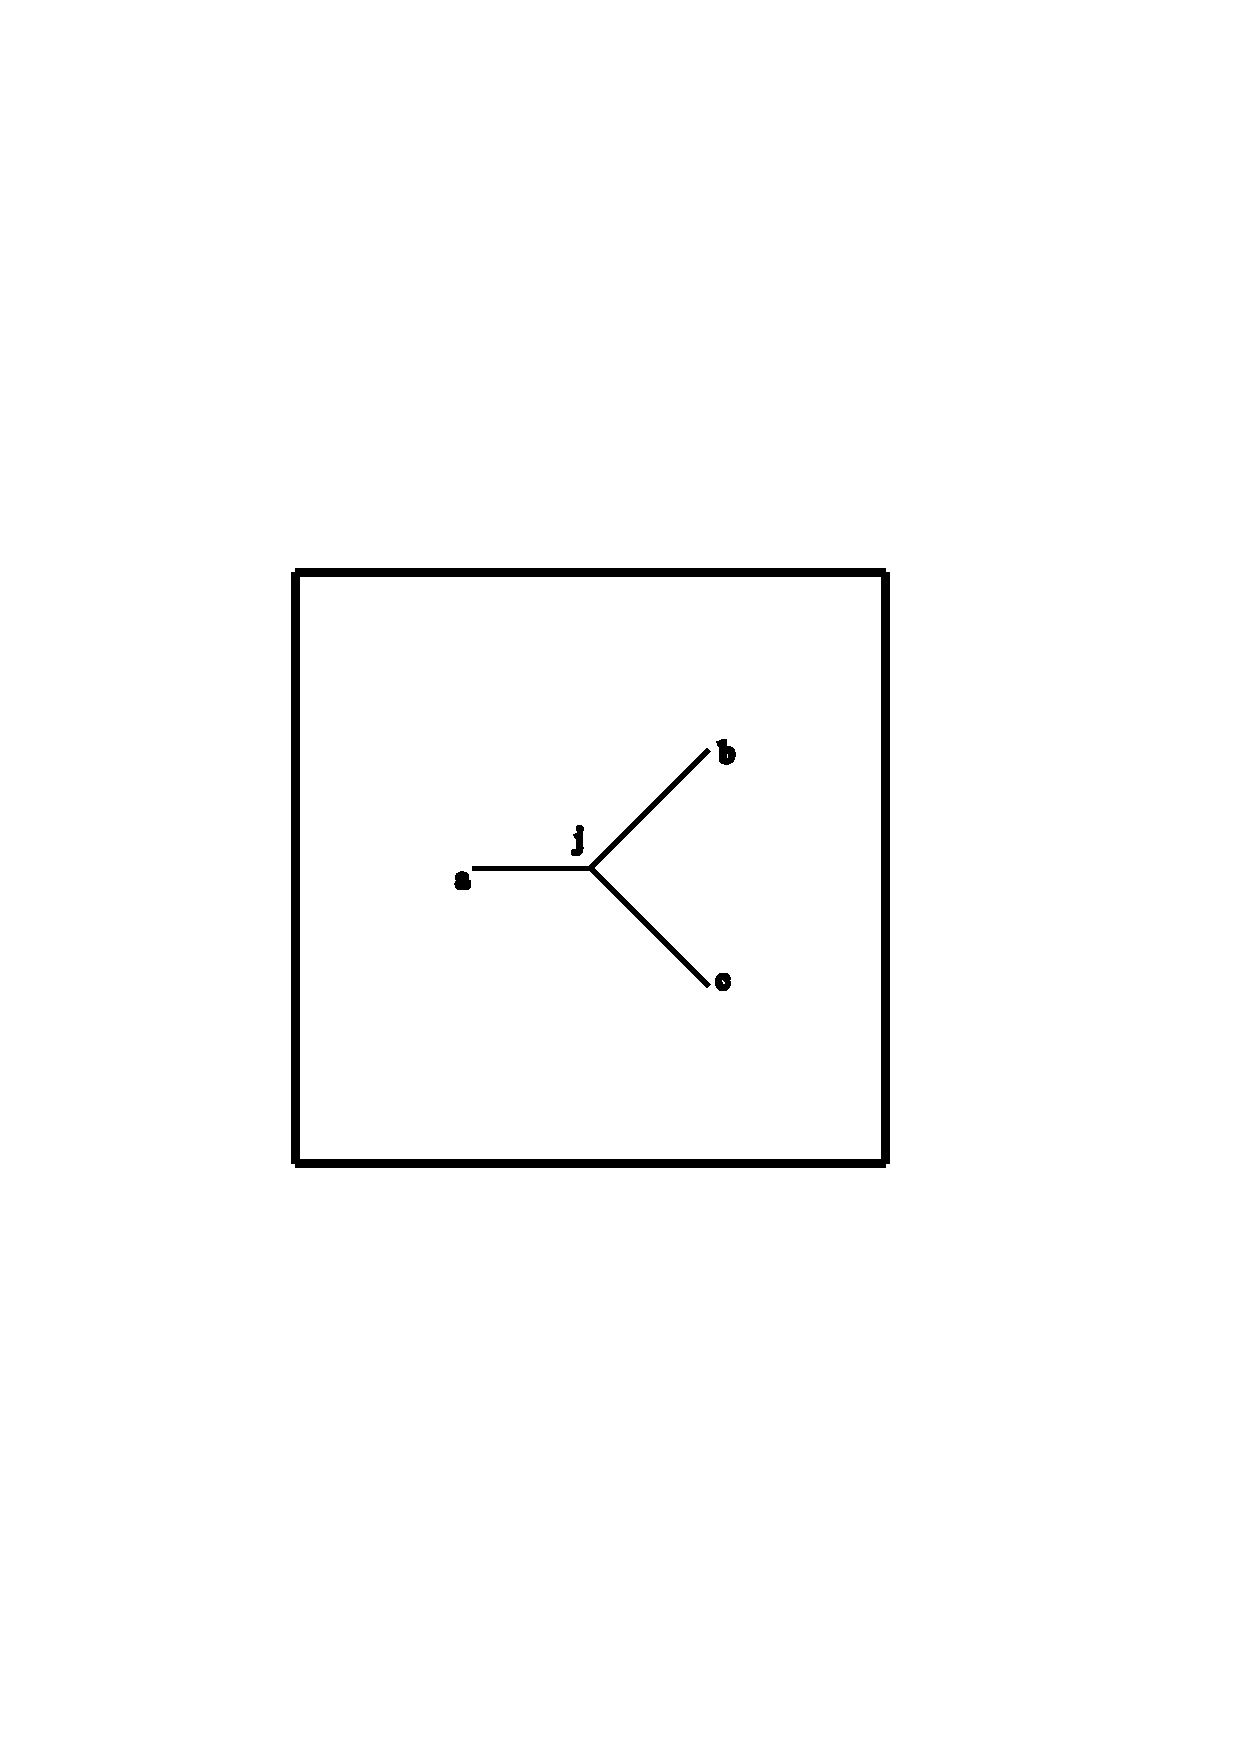
\includegraphics[width=0.3\textwidth]{FigtwoRight.pdf}
			\end{figure}
			%			\item \cite{ambrosio1990approximation} studied the relation between the phase field formulation and its sharp crack limit.
		\end{itemize}
		\item \textbf{Cons:}
		\begin{itemize}
			\item Need to track the complicated geometry of the evolving crack
			\item Need extra input to predict complex phenomena
		\end{itemize}
	\end{itemize}
	\hyperlink{phasefield}{\beamerbutton{The~Smeared~Crack}}
\end{frame}

\begin{frame}[label=subfstvar]
	\frametitle{\SectionTwo}
	\framesubtitle{The first variation}
	%	\vspace{\baselineskip}		
	\begin{itemize}
		\setlength\itemsep{2em}
		\item Taking the first variation yield:
		\begin{multline*}
		\delta \Pi_\ell[(\bm{u}, d), (\bm{w}, q)] :=  \left.\frac{d}{d\epsilon} \Pi_\ell[\bm{u} + \epsilon\bm{w}, d + \epsilon q]\right|_{\epsilon=0} \\
		=\int_\Omega \bm{\sigma}[\bm{\varepsilon}(\bm{u}), d] : \bm{\varepsilon}(\bm{w}) \;d\Omega - \int_{\Gamma_N} \bm{t}_N\cdot \bm{w} \; d\Gamma - \int_\Omega \mathbf{b}\cdot\bm{w} \; d\Omega \\
		\quad - \int_\Omega 2(1-d) q \psi_+(\bm{\varepsilon}) \; d\Omega + 
		g_c\int_\Omega\left(\frac{d\;q}{\ell} + \ell \nabla d\cdot\nabla q\right)\;d\Omega
		\end{multline*}
		where 
		\begin{equation*}
		\bm{\sigma}:=\frac{\partial\psi}{\partial\bm{\varepsilon}} = \left[(1-d)^2 + k\right] \frac{\partial\psi_+(\bm{\varepsilon})}{\partial\bm{\varepsilon}} + \frac{\partial\psi_-(\bm{\varepsilon})}{\partial\bm{\varepsilon}}
		\end{equation*}
		is the Cauchy stress tensor.
	\end{itemize}
	\hyperlink{staticweak}{\beamerbutton{The~weak~form}}
\end{frame}

\begin{frame}[label=subfstvarii]
	\frametitle{\SectionTwo}
	\framesubtitle{The residuals}
	%	\vspace{\baselineskip}		
	\begin{itemize}
		\setlength\itemsep{2em}
		\item If we use $\{\mathbf{N}_P\}$ to denote the set of basis functions for $\bm{u}$ and $\bm{w}$, and $\{\phi_P\}$ that for $d$ and $q$, then we can write the residuals as
		\begin{align*}
		R_P &= \int_\Omega \bm{\sigma}[\bm{\varepsilon}(\bm{u}), d] : \bm{\varepsilon}(\mathbf{N}_P) \;d\Omega - \int_{\Gamma_N} \bm{t}_N\cdot \mathbf{N}_P \; d\Gamma - \int_\Omega \mathbf{b}\cdot\mathbf{N}_P \; d\Omega, \\
		\overline{R}_P &= - \int_\Omega 2(1-d) \phi_P \psi_+(\bm{\varepsilon}) \; d\Omega + 
		g_c\int_\Omega  \left(\frac{d\;\phi_P}{\ell} + \ell \nabla d\cdot\nabla \phi_P\right)\;d\Omega.
		\end{align*}		
	\end{itemize}
	\hyperlink{fenics}{\beamerbutton{FEniCS}}
\end{frame}

\begin{frame}[label=subfstvariii]
	\frametitle{\SectionTwo}
	\framesubtitle{The second variation}
	%	\vspace{\baselineskip}		
	\begin{itemize}
		\setlength\itemsep{2em}
		\item To derive the expression of the tangent stiffness matrices, we take another variation:
		\begin{equation*}
		\begin{aligned}
		\delta^2 \Pi_\ell[(\bm{u}, d), (\bm{w}, q); (\delta\bm{u}, \delta d)] &:=  \left.\frac{d}{d\epsilon} \delta \Pi_\ell[(\bm{u}+\epsilon\delta\bm{u}, d+\epsilon\delta d), (\bm{w}, q)]\right|_{\epsilon=0} \\
		&=\int_\Omega \bm{\varepsilon}(\bm{w}): \mathbb{A}[\bm{\varepsilon}(\bm{u}), d] : \bm{\varepsilon}(\delta\bm{u})  \;d\Omega \\
		&\quad + \int_\Omega 2 q d \left.\frac{\partial \psi_+(\bm{\varepsilon})}{\partial\bm{\varepsilon}}\right|_{\bm{\varepsilon}=\bm{\varepsilon}(\bm{u})} : \bm{\varepsilon}(\delta\bm{u}) \; d\Omega \\
		&\quad + \int_\Omega \bm{\varepsilon}(\bm{w}) : \frac{\partial\bm{\sigma}[\bm{\varepsilon}(\bm{u}), d]}{\partial d} \delta d  \;d\Omega \\
		&\quad - \int_\Omega 2 q \psi_+(\bm{\varepsilon}) \delta d \; d\Omega \\ 
		&\quad + g_c\int_\Omega  \left[\frac{q \delta d}{\ell} + \ell \nabla q \cdot \nabla (\delta d) \right]\;d\Omega.
		\end{aligned}
		\end{equation*}
	\end{itemize}
	\hyperlink{fenics}{\beamerbutton{FEniCS}}
\end{frame}

\begin{frame}[label=subinc]
	\framesubtitle{\SectionTwo}
	\frametitle{Popular Phase Field Models (B)}
	%	\vspace{\baselineskip}		
	\begin{itemize}
		\setlength\itemsep{2em}
		\item \textbf{Model B:} This model assumes that both volumetric expansion and deviatoric deformation contribute to crack propagation but not volumetric compression. \cite{Amor09}
		\begin{align*}
		\psi&=(1-d)^2\psi_{+} + \psi_{-},\quad\sigma=\frac{\partial\psi}{\partial\varepsilon}, \\
		\psi_+&=(\lambda+2\mu/3)\langle \trace \bm{\varepsilon} \rangle_+\bm{1} + 2\mu\dev\bm{\varepsilon},\\
		\psi_-&=(\lambda+2\mu/3)\langle \trace \bm{\varepsilon} \rangle_-\bm{1}.
		\end{align*}
		%		And:
		%		\begin{equation*}
		%		\bm{\sigma}(\bm{\varepsilon}, d) = \frac{\partial\psi}{\partial \bm{\varepsilon}} = (1-d)^2 \frac{\partial\psi_+}{\partial \bm{\varepsilon}} + \frac{\partial\psi_-}{\partial \bm{\varepsilon}}
		%		\end{equation*}
	\end{itemize}
	\hyperlink{RegVarInc}{\beamerbutton{The~incompressibility~formulation}}
\end{frame}

\end{document}

